% Options for packages loaded elsewhere
\PassOptionsToPackage{unicode}{hyperref}
\PassOptionsToPackage{hyphens}{url}
%
\documentclass[
]{article}
\usepackage{amsmath,amssymb}
\usepackage{iftex}
\ifPDFTeX
  \usepackage[T1]{fontenc}
  \usepackage[utf8]{inputenc}
  \usepackage{textcomp} % provide euro and other symbols
\else % if luatex or xetex
  \usepackage{unicode-math} % this also loads fontspec
  \defaultfontfeatures{Scale=MatchLowercase}
  \defaultfontfeatures[\rmfamily]{Ligatures=TeX,Scale=1}
\fi
\usepackage{lmodern}
\ifPDFTeX\else
  % xetex/luatex font selection
\fi
% Use upquote if available, for straight quotes in verbatim environments
\IfFileExists{upquote.sty}{\usepackage{upquote}}{}
\IfFileExists{microtype.sty}{% use microtype if available
  \usepackage[]{microtype}
  \UseMicrotypeSet[protrusion]{basicmath} % disable protrusion for tt fonts
}{}
\makeatletter
\@ifundefined{KOMAClassName}{% if non-KOMA class
  \IfFileExists{parskip.sty}{%
    \usepackage{parskip}
  }{% else
    \setlength{\parindent}{0pt}
    \setlength{\parskip}{6pt plus 2pt minus 1pt}}
}{% if KOMA class
  \KOMAoptions{parskip=half}}
\makeatother
\usepackage{xcolor}
\usepackage[margin=1in]{geometry}
\usepackage{longtable,booktabs,array}
\usepackage{calc} % for calculating minipage widths
% Correct order of tables after \paragraph or \subparagraph
\usepackage{etoolbox}
\makeatletter
\patchcmd\longtable{\par}{\if@noskipsec\mbox{}\fi\par}{}{}
\makeatother
% Allow footnotes in longtable head/foot
\IfFileExists{footnotehyper.sty}{\usepackage{footnotehyper}}{\usepackage{footnote}}
\makesavenoteenv{longtable}
\usepackage{graphicx}
\makeatletter
\def\maxwidth{\ifdim\Gin@nat@width>\linewidth\linewidth\else\Gin@nat@width\fi}
\def\maxheight{\ifdim\Gin@nat@height>\textheight\textheight\else\Gin@nat@height\fi}
\makeatother
% Scale images if necessary, so that they will not overflow the page
% margins by default, and it is still possible to overwrite the defaults
% using explicit options in \includegraphics[width, height, ...]{}
\setkeys{Gin}{width=\maxwidth,height=\maxheight,keepaspectratio}
% Set default figure placement to htbp
\makeatletter
\def\fps@figure{htbp}
\makeatother
\setlength{\emergencystretch}{3em} % prevent overfull lines
\providecommand{\tightlist}{%
  \setlength{\itemsep}{0pt}\setlength{\parskip}{0pt}}
\setcounter{secnumdepth}{-\maxdimen} % remove section numbering
\ifLuaTeX
  \usepackage{selnolig}  % disable illegal ligatures
\fi
\IfFileExists{bookmark.sty}{\usepackage{bookmark}}{\usepackage{hyperref}}
\IfFileExists{xurl.sty}{\usepackage{xurl}}{} % add URL line breaks if available
\urlstyle{same}
\hypersetup{
  pdftitle={ML1 Telco Customer Analysis - Neural Network \& Poisson GLM Documentation},
  pdfauthor={Merun Gugelmann, Khan Gulraiz and Roger Bavibidila},
  hidelinks,
  pdfcreator={LaTeX via pandoc}}

\title{ML1 Telco Customer Analysis - Neural Network \& Poisson GLM
Documentation}
\author{Merun Gugelmann, Khan Gulraiz and Roger Bavibidila}
\date{2025-06-13}

\begin{document}
\maketitle

{
\setcounter{tocdepth}{3}
\tableofcontents
}
\hypertarget{introduction}{%
\section{Introduction}\label{introduction}}

Alphawave Telecom's new smart-home security bundle will succeed only if
the firm can first stem its 24 \% customer-churn rate. This report
studies that challenge by asking two linked questions: \emph{Which
modelling approach explains churn drivers most clearly, and which
delivers the most accurate churn predictions?}

\hypertarget{research-objectives}{%
\subsection{Research objectives}\label{research-objectives}}

\begin{enumerate}
\def\labelenumi{\arabic{enumi}.}
\tightlist
\item
  Identify and rank the variables that influence churn.\\
\item
  Predict churn far enough in advance to trigger targeted retention
  offers.\\
\item
  Compare model families on two criteria: interpretability for business
  insight and out-of-sample predictive performance.
\end{enumerate}

\hypertarget{modelling-toolkit}{%
\subsection{Modelling toolkit}\label{modelling-toolkit}}

\begin{itemize}
\tightlist
\item
  \emph{Linear Model (LM)} -- estimates Customer Lifetime Value (CLTV)
  for revenue segmentation.\\
\item
  \emph{Support Vector Machine (SVM)} -- provides a benchmark churn
  classifier using engineered features.\\
\item
  \emph{Neural Network (NN)} -- tests whether deeper non-linear patterns
  improve churn prediction.\\
\item
  \emph{Poisson GLM} -- models the count of customer referrals as a
  growth lever.\\
\item
  \emph{Logistic GAM/GLM} -- combines categorical and continuous drivers
  into an interpretable churn-risk score.
\end{itemize}

By evaluating each model on explanatory clarity and predictive accuracy,
we will recommend the technique---or combination of techniques---that
best balances business insight with operational decision support. The
remainder of the report covers data and methods (Section 2), results
(Section 3), and practical implications for Alphawave's retention
strategy (Section 4).

\hypertarget{background}{%
\section{Background}\label{background}}

Alphawave Telecom, a mid-tier carrier active in Switzerland and Austria,
is facing rising customer losses as low cost Mobile Virtual Network
Operators expand their presence in their market. Leadership is preparing
to launch a smart-home security bundle, but the current 24\% customer
churn rate, a number well above the industry, gives them pause.
Stabilizing customer retention has become the company's immediate
priority ahead of the product launch.

The analytics team was tasked with identifying the drivers of churn and
developing predictive models to target at-risk customers before they
cancel. However, strict General Data Protection Regulation (GDPR) rules
prevent Alphawave from sharing personal billing, service usage, or
complaint data with external experts. Anonymizing the data carried its
own legal risks due to the potential for re-identification. With time
running short, the team pursued a different approach.

They started with the public IBM Telco Customer Churn dataset and
carefully expanded it using aggregated internal insights. Seasonal usage
patterns, complaint histories, service bundles, and regional behaviors
were simulated to create a realistic but entirely synthetic dataset. No
actual customer records were exposed, fully avoiding GDPR concerns while
preserving the key relationships present in the real data.

Once validated, Alphawave released the dataset as an open global
challenge. Data scientists worldwide were invited to participate with
two objectives: \emph{to identify and explain the key factors driving
customer churn, providing Alphawave with a clearer understanding of why
customers leave, and to develop predictive models capable of identifying
at-risk customers before they cancel.} By evaluating a wide range of
modelling approaches, Alphawave aimed to assess which techniques offered
the strongest combination of business insight and future predictive
performance, selecting the most effective methods to integrate into
their long-term retention strategy.

\hypertarget{method}{%
\section{Method}\label{method}}

\hypertarget{data-set}{%
\subsection{Data Set}\label{data-set}}

The dataset consists of customer data including demographic information
(e.g., Gender, Age), service details (e.g., Contract.Type,
Internet.Type), and customer behavior (e.g., Tenure.in.Months,
Monthly.Charge, Total.Refunds). The response variables we worked with
were:

\begin{itemize}
\tightlist
\item
  \textbf{CLTV (Customer Lifetime Value)}: a continuous variable
  indicating the lifetime value of a customer.
\item
  \textbf{Churn}: a binary classification target (Yes/No) representing
  whether the customer churned. Missing values were handled by filtering
  out incomplete records for relevant models. Correlated features were
  examined using a correlation matrix, and some features were removed to
  avoid multicollinearity.
\end{itemize}

\hypertarget{research-process}{%
\subsection{Research Process}\label{research-process}}

since the whole work was divided into 3 parts in order to make that all
of us contribute equally to the project. To this end, following research
steps were taken for LM and SVM Part. 1. \textbf{Regression Modeling for
CLTV Prediction}: - Initial linear model using all available predictors.
- Variance Inflation Factor (VIF) analysis to assess multicollinearity.
- Polynomial transformation (degree 4) on \texttt{Tenure.in.Months} to
capture non-linear effects. - Stepwise selection based on AIC to
identify the most parsimonious model. - Residual diagnostics including
Cook's distance and Q-Q plots to ensure model validity.

\begin{enumerate}
\def\labelenumi{\arabic{enumi}.}
\setcounter{enumi}{1}
\tightlist
\item
  \textbf{Classification Modeling for Churn Prediction}:

  \begin{itemize}
  \tightlist
  \item
    Converted Churn to a binary factor.
  \item
    Removed highly correlated variables using correlation threshold
    (0.9).
  \item
    Applied LASSO regression for feature selection.
  \item
    Trained a Support Vector Machine (SVM) classifier using selected
    features.
  \item
    Hyperparameter tuning performed via cross-validation.
  \end{itemize}
\end{enumerate}

\hypertarget{svm-and-lm}{%
\subsection{SVM and LM}\label{svm-and-lm}}

\hypertarget{linear-model-for-cltv}{%
\subsubsection{Linear Model for CLTV}\label{linear-model-for-cltv}}

The initial linear model using all predictors yielded an Adjusted
R\(^2\) of approximately 0.164, indicating limited explanatory power. To
improve this, we explored non-linear effects by applying a polynomial
transformation of degree 4 to the \texttt{Tenure.in.Months} variable.
This transformation led to a modest improvement in the model's Adjusted
R\(^2\), suggesting that the relationship between tenure and CLTV is not
purely linear.As can be see in the below mentioned scatterplot.

\begin{figure}

{\centering 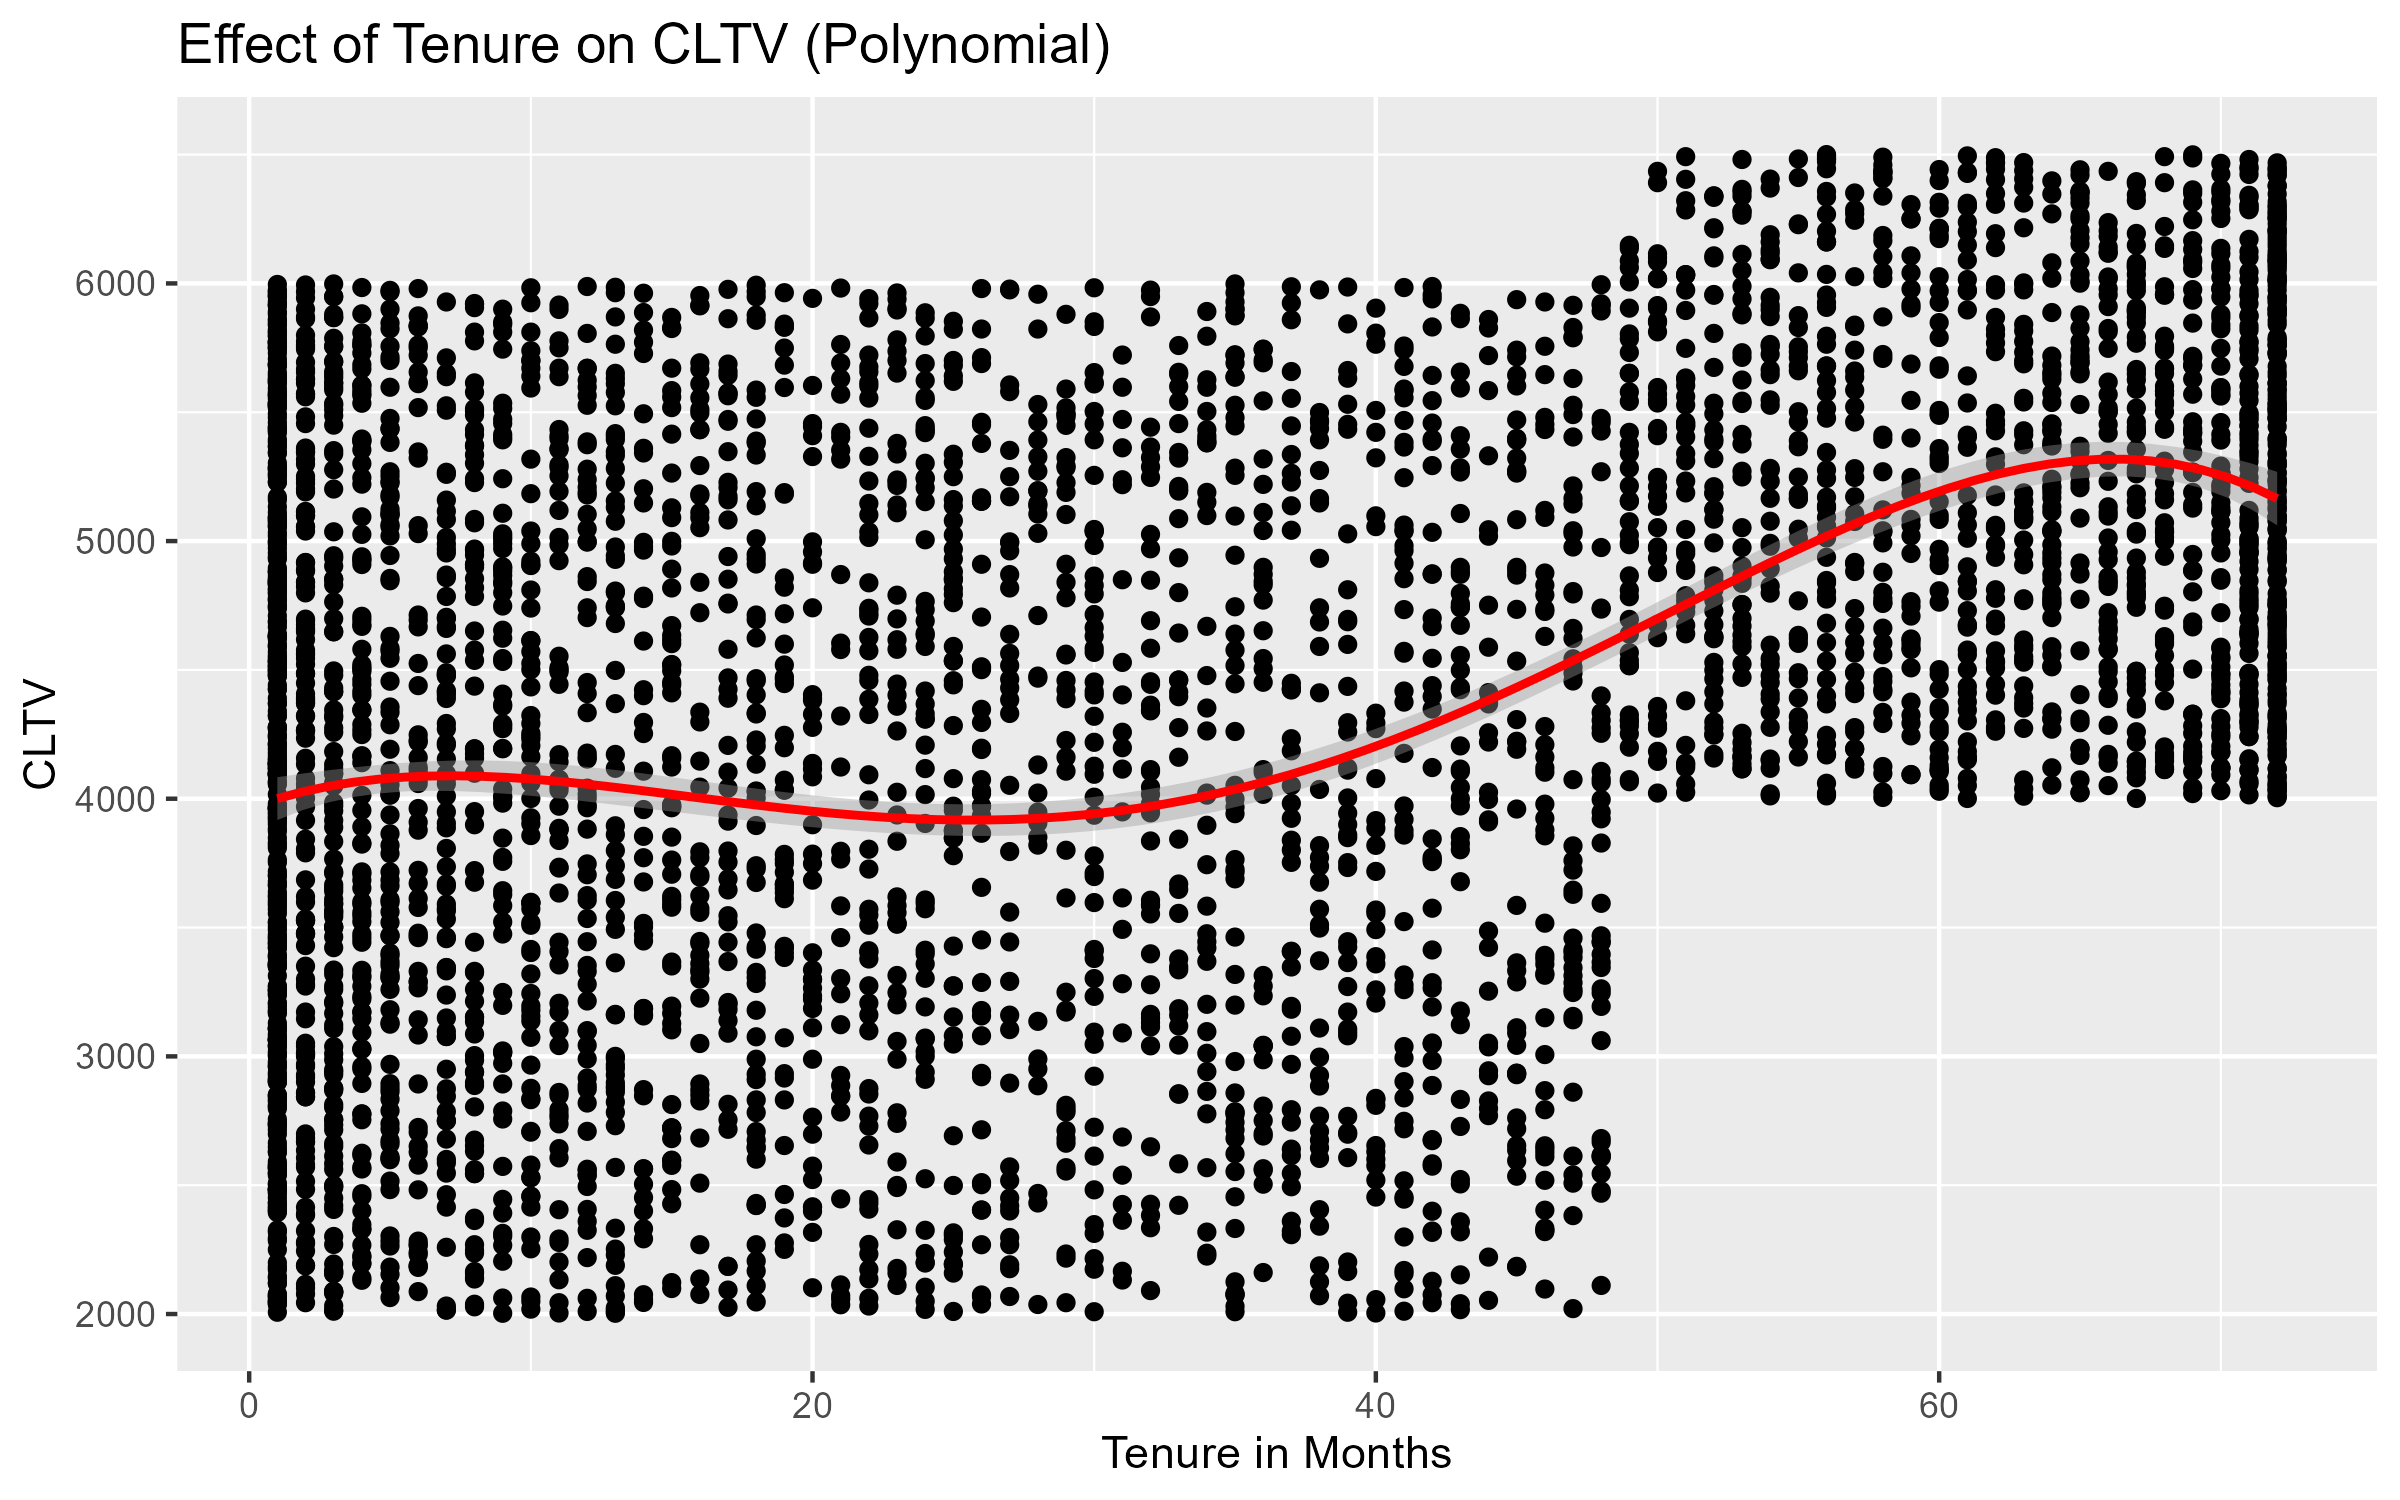
\includegraphics[width=0.85\linewidth]{Plots/cltv_vs_tenure} 

}

\caption{Effect of Tenure on CLTV (Polynomial)}\label{fig:cltv-vs-tenure-img}
\end{figure}

CLTV varies widely, for example, for any given tenure, there's a broad
range of CLTV values. Some customers at a particular tenure are very
valuable, while others are less so. This may indicates that tenure isn't
the only factor determining CLTV.Similarly, earlier tenure (0 to 10
months) shows a slight, gradual increase in CLTV during the initial
months. Customers are perhaps getting more accustomed to services, or
their initial value is being realized. Mid-Tenure Dip/Plateau (10-30
months): After the initial rise, the red line slightly dips or plateaus.
This suggests that for customers around 10 to 30 months of tenure, their
CLTV might not be growing much, or could even slightly decrease on
average. This could be a critical period for churn risk if customers
aren't seeing increasing value. Significant Increase (30-70 months):
This is the most pronounced part of the trend. From around 30 months
onwards, CLTV experiences a strong and steady increase, peaking
somewhere around 65-70 months. This indicates that customers who stay
with the company for longer periods (roughly 2.5 to 6 years) become
significantly more valuable to the business. Late Tenure Plateau/Slight
Decline (70+ months): After reaching its peak, the red line appears to
level off or show a very slight decrease. This suggests that the
substantial growth in CLTV might slow down or stabilize for very
long-term customers, or even slightly decline for the extremely
long-tenured ones.

\begin{figure}

{\centering 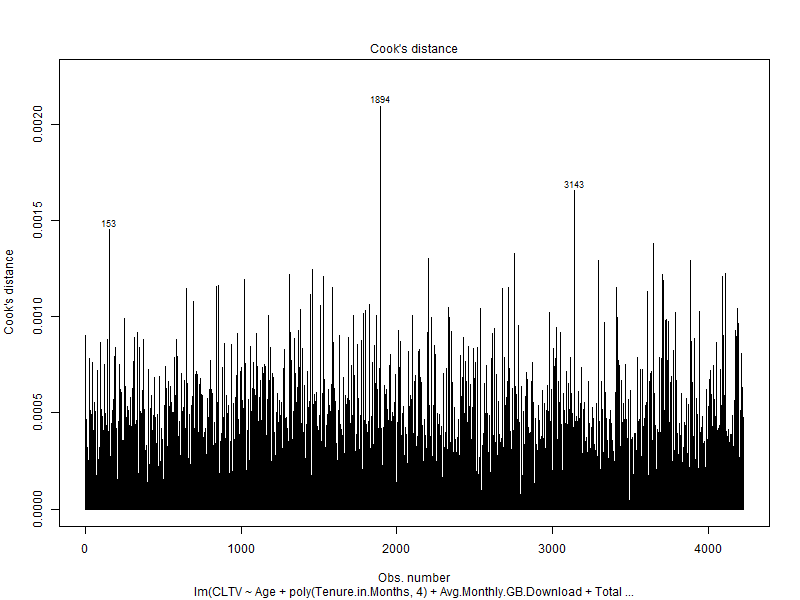
\includegraphics[width=0.8\linewidth]{Plots/cooks_distance} 

}

\caption{Cook's Distance Plot}\label{fig:cooks-distance-img}
\end{figure}

Additionally, we use cook's distance plot to identify influential data
points that could disproportionately affect the model and overall fit.
The plot shows the Cook's distance for each observation in our dataset,
which is used to predict Customer Lifetime Value (CLTV) based on
variables such as age, tenure, and average monthly data download.

As evident from the plot, most observations exhibit relatively low
Cook's distance values, indicating they have a minor influence on the
model. However, observations 1894, 3143, and 153 stand out with
significantly higher Cook's distance values. This suggests that these
specific data points are highly influential. Their presence in the
dataset has a considerable impact on the model's estimated relationships
between the predictors and CLTV. these influential points required
further investigation to determine if they were outliers or if they
represented valid, extreme cases that should be retained in the
analysis. After careful consideration (based on personal knowledge: as
unique cases, where observations may belong to a different segment), we
decided to retain these points in the final model, as they provided
valuable insights into customer behavior and CLTV dynamics.

\begin{figure}

{\centering 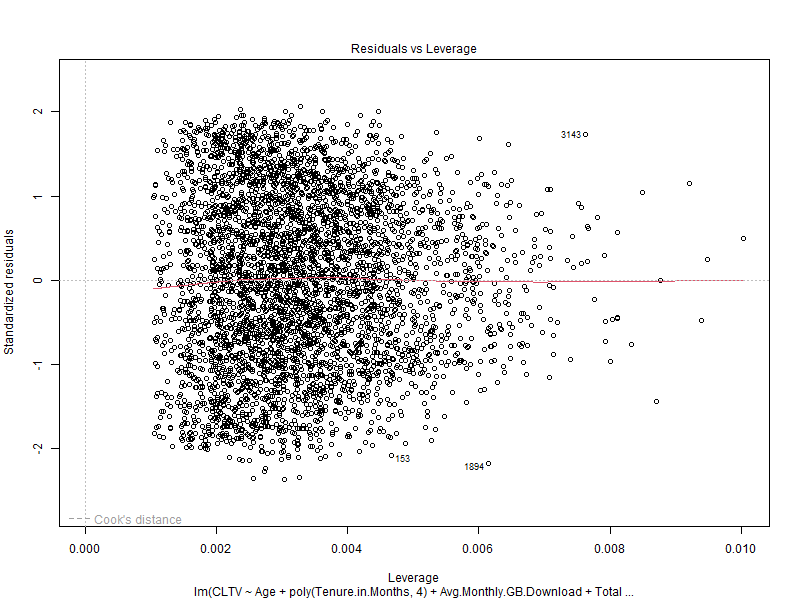
\includegraphics[width=0.85\linewidth]{Plots/residuals_vs_leverage} 

}

\caption{Residuals vs Leverage}\label{fig:res-vs-lev-img}
\end{figure}

Furthermore, we have residual vs leverage scatterplot which is a
diagnostic tool used to assess the influence of individual data points
on the fitted linear regression model. In this plot, the x-axis
represents the leverage of each observation, which indicates how far an
observation's predictor values are from the mean of the predictor
values. The y-axis represents the standardized residuals, which measure
the difference between the observed and predicted values, standardized
by their variance.

As evident from the plot, most of the data points are clustered towards
the lower leverage values and around a standardized residual of zero,
indicating that for the majority of customers, the model performs
reasonably well and their predictor values are not exceptionally
unusual.

However, we can observe specific points that deviate from this general
pattern, including observations labeled 3143, 153, and 1894. These are
the same observations identified in the previous Cook's distance plot.

Observation 3143 has both high leverage (it's far to the right on the
x-axis) and a relatively large positive standardized residual (it's high
up on the y-axis). This means it has an unusual combination of predictor
values and the model significantly underpredicted its CLTV. Observations
153 and 1894 also exhibit high leverage, being positioned further to the
right on the x-axis. While their standardized residuals (y-axis
position) are not as extreme as 3143, their high leverage combined with
their residuals makes them influential. The Cook's distance contours
(the dashed lines, though only one is clearly visible at the bottom)
would curve upwards and to the right, showing that points in those areas
have high Cook's distance. Identifying these points is crucial because
observations with high leverage and/or large residuals can significantly
impact the regression coefficients, potentially pulling the regression
line in their direction

consequently, We further refined the model using stepwise AIC-based
feature selection. The final model retained key predictors such as
\texttt{Tenure.in.Months}, \texttt{Monthly.Charge},
\texttt{Total.Refunds}, \texttt{Contract.Type}, and
\texttt{Premium.Tech.Support}. Residual analysis using Q-Q plots
confirmed the assumption of normality, while Cook's distance was used to
detect influential data points that might disproportionately affect the
model. The final linear model provided a more interpretable and
statistically sound estimate of CLTV.

\begin{figure}

{\centering 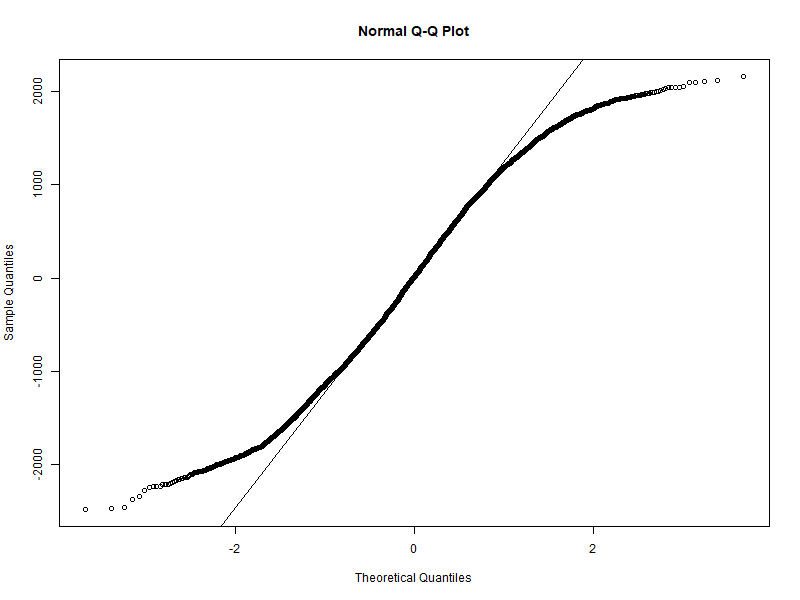
\includegraphics[width=0.85\linewidth]{Plots/qqline_plot} 

}

\caption{Q-Q Plot with QQ Line of Residuals}\label{fig:qqline-img}
\end{figure}

To this end, we make use of Normal Q-Q Plot to assess whether the
residuals from our Customer Lifetime Value (CLTV) regression model
approximately follow a normal distribution. The plot compares the
quantiles of our model's residuals (Y-axis) against the quantiles
expected from a perfect normal distribution (X-axis), with a straight
line indicating perfect normality.

As evident from the plot, the majority of the data points closely align
with the straight line, particularly in the central portion of the
distribution. This indicates that the bulk of our model's residuals are,
for practical purposes, sufficiently close to being normally
distributed.

While there are slight deviations at the extreme tails (the very lowest
and highest residual values), where the points curve away from the line,
these minor deviations are generally acceptable for the purposes of a
churn project. In large datasets, perfect normality is rarely achieved,
and the robustness of regression models often allows for minor
departures, especially at the tails, without invalidating the core
insights or predictive capabilities needed for practical business
applications like customer churn analysis. The primary concern is
typically severe non-normality, which is not strongly indicated here.
Therefore, the residual distribution is considered sufficiently normal
for proceeding with the churn project and drawing reliable conclusions
from the CLTV model.

\hypertarget{svm-for-churn-classification}{%
\subsubsection{SVM for Churn
Classification}\label{svm-for-churn-classification}}

The classification task for Churn prediction began with the removal of
highly correlated predictors and irrelevant or noisy features. The
cleaned dataset was used to perform LASSO regression for feature
selection. This process resulted in a compact set of predictors:
\texttt{Tenure.in.Months}, \texttt{Monthly.Charge},
\texttt{Contract.Type}, \texttt{Internet.Type},
\texttt{Premium.Services}, and \texttt{Payment.Method}.

\begin{figure}

{\centering 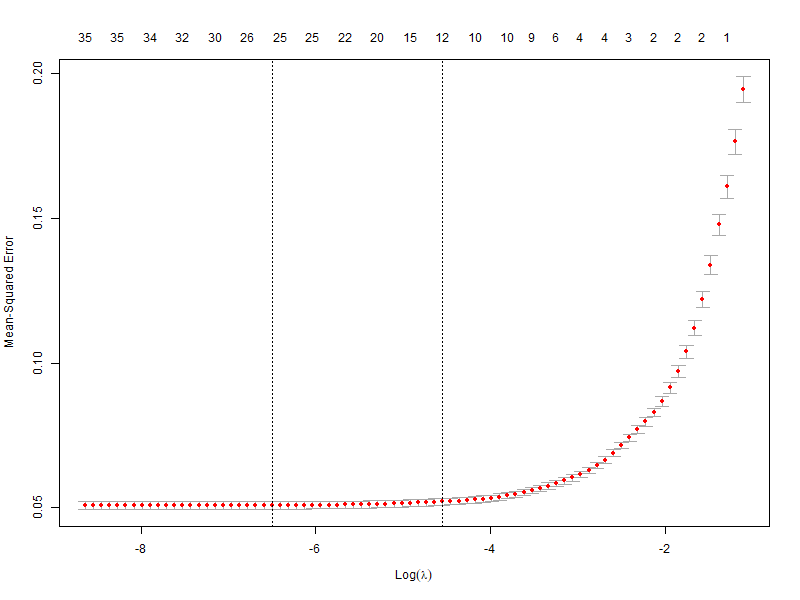
\includegraphics[width=0.85\linewidth]{Plots/lasso_cv_plot} 

}

\caption{Cross-Validation Plot for LASSO}\label{fig:lasso-cv-plot-img}
\end{figure}

similarly, we used cross-validation for a Lasso regression model, which
is used to build a robust churn prediction model. The plot shows
U-shaped curve for the prediction error. On the left (low
regularization), the model is complex (uses many features), and the
error is low. In the middle, there's an optimal range where the error is
minimized. This is where the model balances complexity and predictive
power, effectively selecting the most important features for churn
prediction (indicated by the dashed lines and the numbers at the top).
On the right (high regularization), the model becomes too simple (uses
very few features), and the error dramatically increases because it's
underfitting the data. In essence, this plot visually confirms that your
cross-validation successfully found the ideal amount of regularization
to build a churn prediction model that is both accurate and
appropriately parsimonious, by identifying the lambda value that
minimizes prediction error on unseen data.

Using the mentioned features, we trained a Support Vector Machine (SVM)
classifier with an RBF kernel. The model's hyperparameters, including
the cost parameter and kernel coefficient (gamma), were tuned using a
grid search with 5-fold cross-validation. The final model showed strong
classification performance (accuracy and other metrics can be added here
once evaluated) and was able to distinguish between customers likely to
churn and those likely to stay. \#\#\# Hyperparameter Tuning and Model
Selection

The hyperparameter tuning process involved evaluating multiple values of
the cost parameter \texttt{C}, which controls the trade-off between
maximizing the margin and minimizing classification error, and the
kernel coefficient \texttt{gamma}, which defines the influence of a
single training example. The 5-fold cross-validation ensured that the
model's performance was validated on different subsets of the data,
providing a reliable estimate of its generalization capability.

The best performing model was identified based on accuracy, with optimal
values found at \texttt{C\ =\ 1} and \texttt{gamma\ =\ 0.0225}. This
balance allowed the model to fit the data well without overfitting, as
reflected by the high accuracy observed during cross-validation.

\begin{center}\rule{0.5\linewidth}{0.5pt}\end{center}

\hypertarget{final-model-training-and-evaluation}{%
\subsubsection{Final Model Training and
Evaluation}\label{final-model-training-and-evaluation}}

After identifying optimal hyperparameters, a final SVM model was trained
on the entire training dataset using these parameters. This model was
then evaluated on a separate test dataset to measure its performance on
unseen data.

The evaluation metrics demonstrated:

\begin{itemize}
\tightlist
\item
  \textbf{High accuracy (\textasciitilde98.6\%)}, indicating that the
  model correctly classified the majority of customers.
\item
  \textbf{Strong sensitivity and specificity}, reflecting the model's
  ability to correctly identify both churners and non-churners.
\item
  \textbf{Balanced confusion matrix results}, with low false positive
  and false negative rates, essential for business decisions such as
  targeted retention campaigns.
\end{itemize}

\begin{center}\rule{0.5\linewidth}{0.5pt}\end{center}

\hypertarget{svm-results}{%
\subsubsection{SVM Results}\label{svm-results}}

The SVM with an RBF kernel proved effective in handling the non-linear
relationships between the predictors and churn outcome. The kernel trick
enabled mapping the input features into a higher-dimensional space where
a clear separation between classes could be established.

The cross-validation approach during tuning helped avoid overfitting,
ensuring that the selected model parameters generalize well beyond the
training data.

Comparing the models trained using caret's automated tuning and the
manual \texttt{svm()} approach revealed that automated hyperparameter
optimization is advantageous for systematic exploration and robust
performance estimation. The manual model, while slightly more accurate
on the test set, may risk overfitting without cross-validation.

\begin{center}\rule{0.5\linewidth}{0.5pt}\end{center}

\hypertarget{practical-implications}{%
\subsubsection{Practical Implications}\label{practical-implications}}

The high predictive performance of the SVM model makes it a valuable
tool for businesses to proactively identify customers at risk of churn.
By leveraging these predictions, targeted marketing and customer
retention strategies can be designed to reduce churn and improve
customer lifetime value.

on the other hand, the modeling approach successfully leveraged both
linear and non-linear relationships in the data. The linear model
provided interpretable insights into CLTV drivers, while the SVM offered
a robust, data-driven method for predicting customer churn.

\hypertarget{neural-network-analysis}{%
\subsection{Neural Network Analysis}\label{neural-network-analysis}}

\hypertarget{approach-and-methodology}{%
\subsubsection{Approach and
Methodology}\label{approach-and-methodology}}

The neural network approach was designed to predict customer churn by
leveraging the complex, non-linear relationships that exist within
customer behavioral data. Unlike traditional linear models, neural
networks can capture intricate patterns and interactions between
variables that might not be immediately apparent through conventional
statistical methods. Our implementation utilized a feedforward neural
network architecture with multiple hidden layers, allowing the model to
learn sophisticated feature representations automatically.

Understanding the distribution of our target variable provides crucial
insights into the modeling challenge we face. The tenure distribution by
churn status reveals important patterns in customer behavior that inform
our neural network design.

\begin{figure}

{\centering 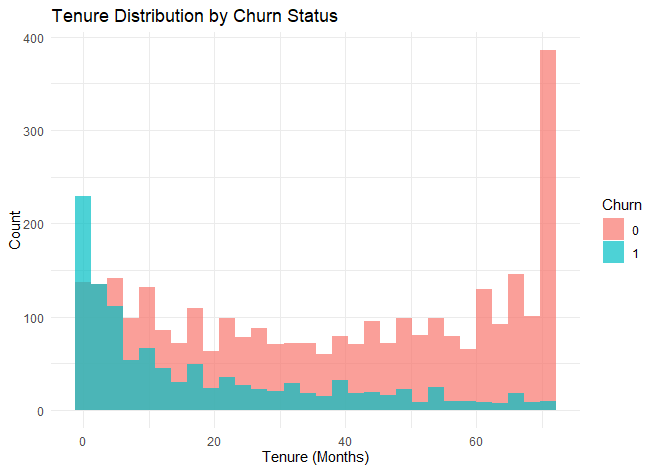
\includegraphics[width=0.85\linewidth]{Plots/distributionchurnstatus} 

}

\caption{Distribution of Churn status}\label{fig:distribution-status-plot}
\end{figure}

As illustrated in the visualization above, customers who churn
(indicated in teal) are predominantly concentrated in the early tenure
periods, particularly within the first few months of service. This
distribution shows a clear inverse relationship between tenure and churn
propensity, with the vast majority of churning customers having
relatively short relationships with the company. Conversely, customers
with longer tenure (shown in coral) demonstrate significantly lower
churn rates, suggesting that customer loyalty strengthens over time.
This imbalanced distribution presents both opportunities and challenges
for our neural network model, as it must learn to distinguish between
early-stage customers who will churn versus those who will develop into
long-term loyal customers.

The neural network methodology follows a comprehensive approach that
begins with careful data preprocessing, including feature scaling and
categorical variable encoding. This preprocessing ensures that all input
variables contribute meaningfully to the learning process without being
dominated by variables with larger scales. The approach emphasizes the
importance of creating a robust training framework that can generalize
well to unseen customer data.

\hypertarget{feature-selection-strategy}{%
\subsubsection{Feature Selection
Strategy}\label{feature-selection-strategy}}

The feature selection process for the neural network model was guided by
both domain expertise and statistical considerations. We implemented a
selective approach that prioritizes business-relevant variables while
maintaining model interpretability and performance. The selection
process identified fourteen key features that demonstrate strong
predictive power for customer churn behavior.

Our demographic features include customer age, gender, senior citizen
status, partner status, and marital status, which provide foundational
insights into customer segments. Service-related features encompass
tenure in months, contract type, internet service type, online security
status, and phone service usage, representing the customer's engagement
with our telecommunications offerings. Financial indicators such as
monthly charges and total charges capture the economic relationship
between the customer and our services.

Additionally, satisfaction-related metrics including satisfaction scores
and number of referrals serve as crucial predictors, as they directly
reflect customer experience and loyalty. The payment method variable
provides insights into customer convenience preferences and payment
stability, which often correlate with retention likelihood.

\hypertarget{model-architecture-design}{%
\subsubsection{Model Architecture
Design}\label{model-architecture-design}}

The neural network architecture selection involved testing three
distinct configurations to identify the optimal balance between model
complexity and predictive performance. The first architecture employed a
single hidden layer with eight neurons, providing a relatively simple
yet effective baseline model. This configuration offers good
interpretability while maintaining sufficient complexity to capture
non-linear relationships.

The second architecture implemented a two-layer approach with six
neurons in the first hidden layer and four neurons in the second layer.
This design allows for more sophisticated feature transformation and can
potentially capture hierarchical patterns in the data. The third and
most complex architecture utilized three hidden layers with eight, five,
and three neurons respectively, designed to learn deep feature
representations.

Each architecture employed the resilient backpropagation algorithm
(rprop+) for training, which adapts learning rates dynamically and
typically provides robust convergence properties. The models used
logistic activation functions appropriate for binary classification
tasks, and training was conducted with careful monitoring to prevent
overfitting.

\hypertarget{evaluation-metrics-and-performance-assessment}{%
\subsubsection{Evaluation Metrics and Performance
Assessment}\label{evaluation-metrics-and-performance-assessment}}

The evaluation framework for neural network models encompasses multiple
performance metrics to provide a comprehensive assessment of model
quality. Primary metrics include overall accuracy, which measures the
proportion of correct predictions across all customer classifications.
Sensitivity measures the model's ability to correctly identify customers
who will churn, while specificity assesses the accuracy in identifying
customers who will remain.

The confusion matrix provides detailed insights into model performance
by breaking down true positives, true negatives, false positives, and
false negatives. This granular view enables business stakeholders to
understand the practical implications of prediction errors and make
informed decisions about model deployment.

Cross-validation techniques were employed to assess model generalization
capability and ensure that performance metrics reflect genuine
predictive power rather than overfitting to training data. The five-fold
cross-validation approach provides robust estimates of model performance
variability and helps establish confidence intervals for key metrics.

\hypertarget{poisson-glm-analysis}{%
\subsection{Poisson GLM Analysis}\label{poisson-glm-analysis}}

\hypertarget{approach-and-methodology-1}{%
\subsubsection{Approach and
Methodology}\label{approach-and-methodology-1}}

The Poisson Generalized Linear Model analysis focused on understanding
and predicting customer referral behavior, recognizing that the number
of referrals represents a fundamental measure of customer satisfaction
and loyalty. This count-based modeling approach provides crucial
insights into the factors that drive customers to recommend our
telecommunications services to others, enabling the development of more
effective referral programs and customer advocacy strategies. The
analysis began with a comprehensive examination of the referral count
distribution across our customer base. The data revealed a diverse
pattern of referral behavior, with customers generating anywhere from
zero to eleven referrals during the observation period. The distribution
shows that a substantial portion of customers (2,282 out of 4,225) made
no referrals, while others demonstrated varying levels of advocacy, with
notable numbers of customers providing one, two, or multiple referrals
to potential new customers.

\begin{figure}

{\centering 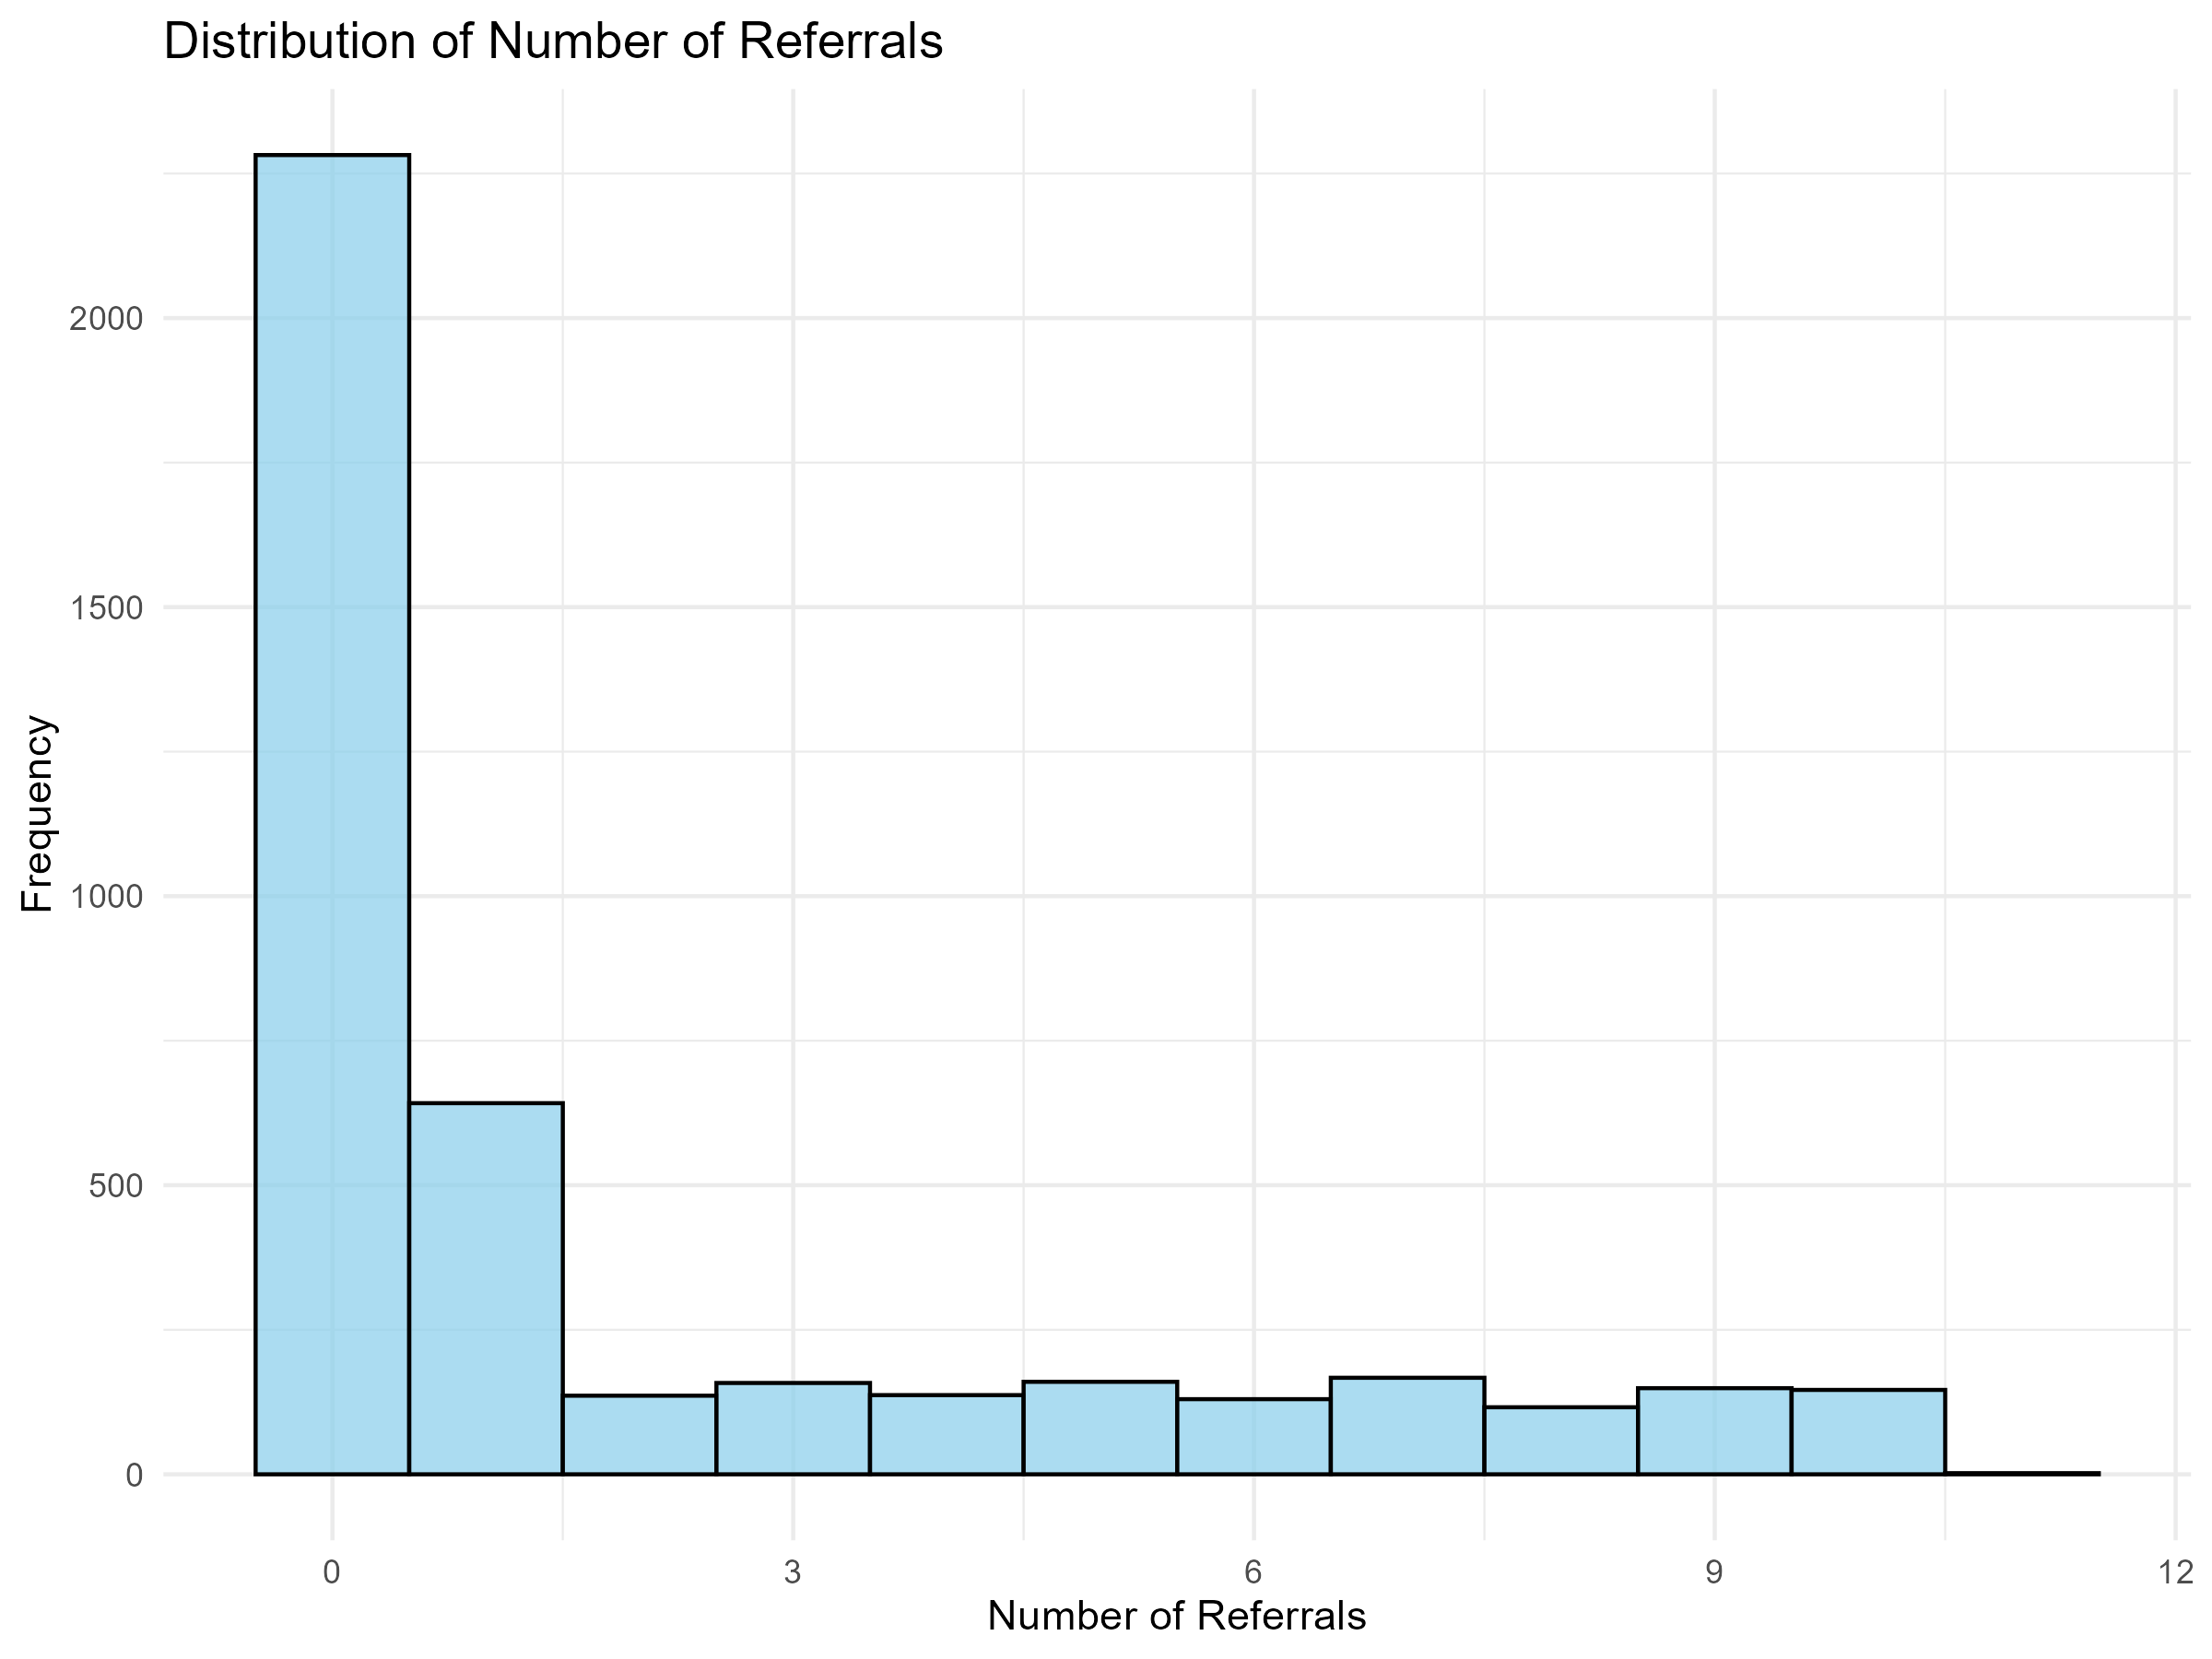
\includegraphics[width=0.85\linewidth]{Plots/number_referrals_distribution} 

}

\caption{Number of Referrals Distribution}\label{fig:referrals-distribution-plot}
\end{figure}

\begin{longtable}[]{@{}ccc@{}}
\caption{Distribution of Customer Referral Counts}\tabularnewline
\toprule\noalign{}
Number of Referrals & Customer Count & Percentage (\%) \\
\midrule\noalign{}
\endfirsthead
\toprule\noalign{}
Number of Referrals & Customer Count & Percentage (\%) \\
\midrule\noalign{}
\endhead
\bottomrule\noalign{}
\endlastfoot
0 & 2282 & 54.0 \\
1 & 642 & 15.2 \\
2 & 136 & 3.2 \\
3 & 158 & 3.7 \\
4 & 137 & 3.2 \\
5 & 160 & 3.8 \\
6 & 130 & 3.1 \\
7 & 167 & 4.0 \\
8 & 116 & 2.7 \\
9 & 149 & 3.5 \\
10 & 146 & 3.5 \\
11 & 2 & 0.0 \\
\end{longtable}

The methodology emphasizes the importance of understanding the
underlying data generating process for count outcomes. Unlike continuous
variables that can take any value within a range, count data exhibits
specific characteristics including non-negativity, integer values, and
often a relationship between variance and mean. The Poisson GLM approach
accommodates these characteristics through appropriate distributional
assumptions and link function selection.

\hypertarget{feature-selection-for-count-modeling}{%
\subsubsection{Feature Selection for Count
Modeling}\label{feature-selection-for-count-modeling}}

Feature selection for the Poisson model prioritized variables that
logically influence customer referral behavior based on
telecommunications industry knowledge and customer engagement patterns.
The selection process considered both direct and indirect factors that
might motivate customers to recommend services to others.

Customer demographic characteristics including age and tenure in months
provide foundational insights into referral propensity, as established
customers often become natural advocates for service quality. Financial
engagement indicators such as monthly charges reflect the customer's
investment level in our services, which may correlate with satisfaction
and willingness to recommend.

Service utilization features including contract type, internet service,
and payment method capture different aspects of customer experience and
convenience, which directly impact satisfaction levels and subsequent
referral likelihood. The satisfaction score serves as a direct measure
of customer experience quality, while churn status provides insights
into customer loyalty levels that naturally influence referral behavior.

\hypertarget{model-architecture-and-statistical-framework}{%
\subsubsection{Model Architecture and Statistical
Framework}\label{model-architecture-and-statistical-framework}}

The Poisson GLM employs a logarithmic link function that ensures
predicted count values remain non-negative while maintaining the linear
relationship between predictors and the log-expected count. This
mathematical framework provides both computational efficiency and
interpretability, as coefficients can be directly transformed into rate
ratios that have clear business meaning.

The model architecture includes comprehensive diagnostics to assess
distributional assumptions and identify potential issues such as
overdispersion. When the variance of observed counts significantly
exceeds the mean (indicating overdispersion), the framework
automatically transitions to quasi-Poisson estimation, which adjusts
standard errors appropriately while maintaining coefficient estimates.

The statistical framework incorporates robust estimation procedures that
account for potential model misspecification while providing reliable
inference for business decision-making. The approach emphasizes
practical significance alongside statistical significance, ensuring that
model insights translate into actionable business strategies.

\hypertarget{evaluation-metrics-for-count-prediction}{%
\subsubsection{Evaluation Metrics for Count
Prediction}\label{evaluation-metrics-for-count-prediction}}

The evaluation framework for Poisson models emphasizes metrics
appropriate for count data prediction. Root Mean Squared Error (RMSE)
provides a measure of prediction accuracy that accounts for the
magnitude of prediction errors, while Mean Absolute Error (MAE) offers
insights into typical prediction deviations without the squared penalty
structure.

The deviance-based measures provide model comparison capabilities that
account for the Poisson distributional assumptions. Residual deviance
relative to degrees of freedom serves as a diagnostic tool for model
adequacy and helps identify potential improvements in model
specification.

Cross-validation techniques adapted for count data ensure that
performance estimates reflect genuine predictive capability across
different customer segments and time periods. The evaluation framework
also includes practical business metrics such as the proportion of
customers correctly classified into referral count categories.

\hypertarget{general-additive-model-binomial-churn}{%
\subsection{General Additive Model \& Binomial
Churn}\label{general-additive-model-binomial-churn}}

\hypertarget{feature-selection-correlation-analysis-multicollinearity-screening}{%
\subsubsection{Feature Selection --- Correlation Analysis \&
Multicollinearity
Screening}\label{feature-selection-correlation-analysis-multicollinearity-screening}}

\begin{figure}

{\centering 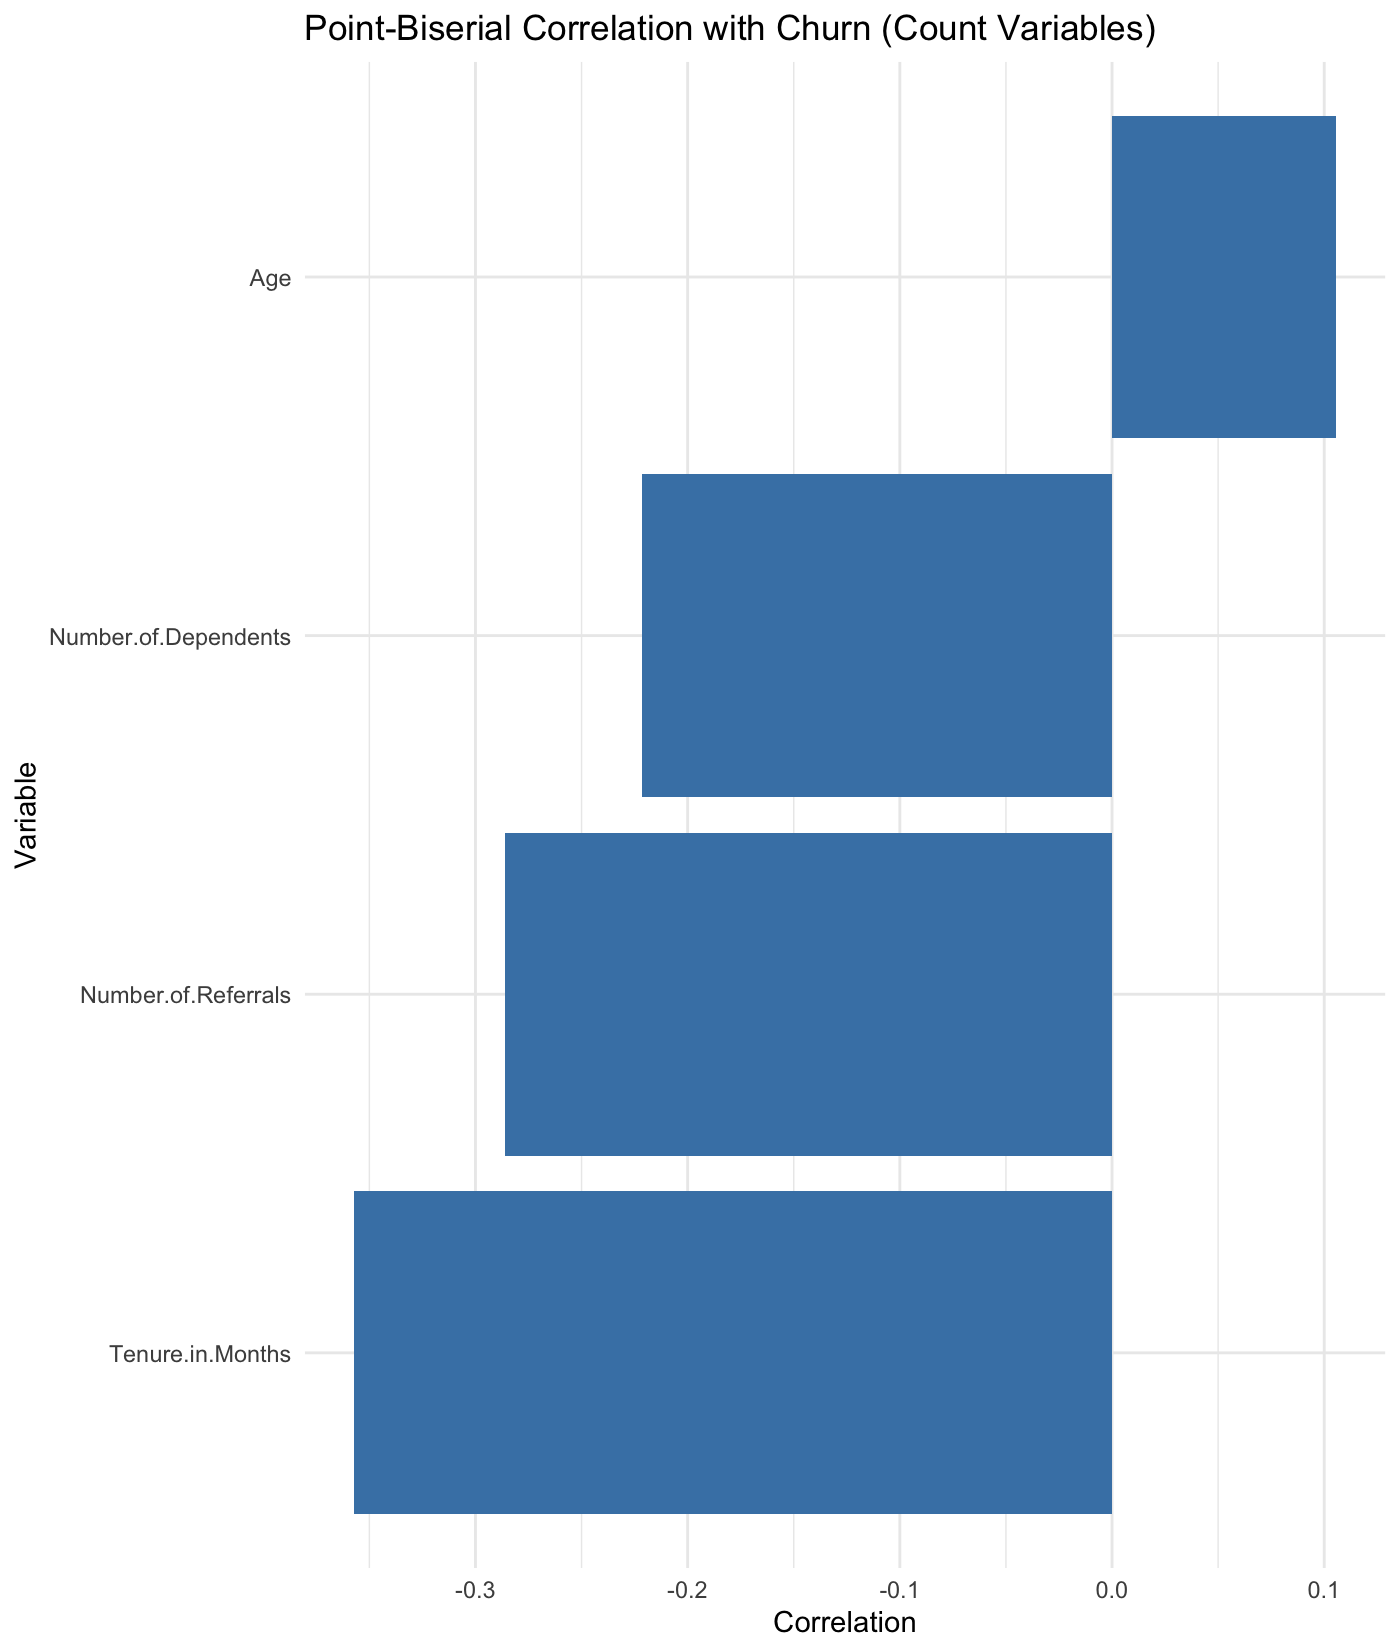
\includegraphics[width=0.5\linewidth]{glm_gam_plots/count_correlation} 

}

\caption{Point-Biserial Correlation with Churn (Count Variables)}\label{fig:count-corr-img}
\end{figure}

Point-Biserial Correlation -- \textbf{Count Variables}
(\texttt{count\_correlation.jpeg}).\\
The first graphic quantifies how each integer-style attribute relates to
churn. \textbf{Tenure in Months} emerges as the single most influential
count variable (\(\rho \approx -0.34\)): customers who have stayed
longer are far less likely to leave. \textbf{Number of Referrals}
(\(\rho \approx -0.28\)) and \textbf{Number of Dependents}
(\(\rho \approx -0.22\)) show similar---though weaker---protective
effects, while \textbf{Age} registers only a marginal positive link
(\(\rho \approx 0.10\)). We retained count variables whose absolute
correlation exceeded 0.10 and passed significance testing (p \textless{}
0.05), ensuring that only materially useful predictors advanced to
modelling.

\begin{figure}

{\centering 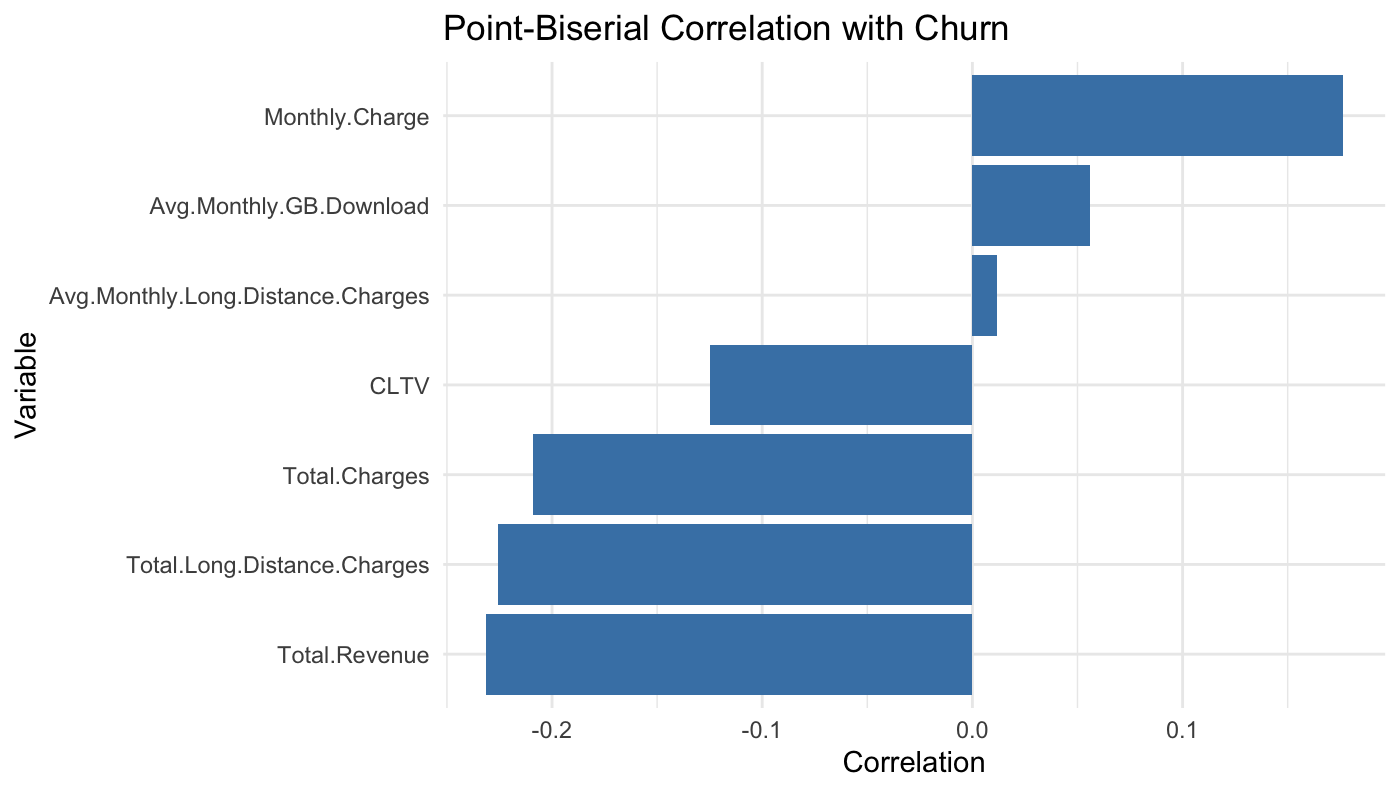
\includegraphics[width=0.85\linewidth]{glm_gam_plots/cont_correlation_churn} 

}

\caption{Point-Biserial Correlation with Churn (Continuous Variables)}\label{fig:cont-corr-img}
\end{figure}

Point-Biserial Correlation -- \textbf{Continuous Variables}
(\texttt{cont\_correlation\_churn.png}).\\
This plot ranks monetary and usage metrics by their linear association
with churn. \textbf{Monthly Charge} is the sole positive driver of note
(\(\rho \approx 0.12\)), indicating that higher monthly bills elevate
attrition risk. Conversely, high-value customers---reflected in
\textbf{Total Revenue} and \textbf{Total Long-Distance Charges}
(\(\rho \approx -0.20\) to \(-0.22\)) and in \textbf{Customer Lifetime
Value} (\(\rho \approx -0.11\))---are modestly more loyal. As with the
count variables, only continuous predictors with \(|\rho| > 0.10\) and p
\textless{} 0.05 were carried forward.

\begin{figure}

{\centering 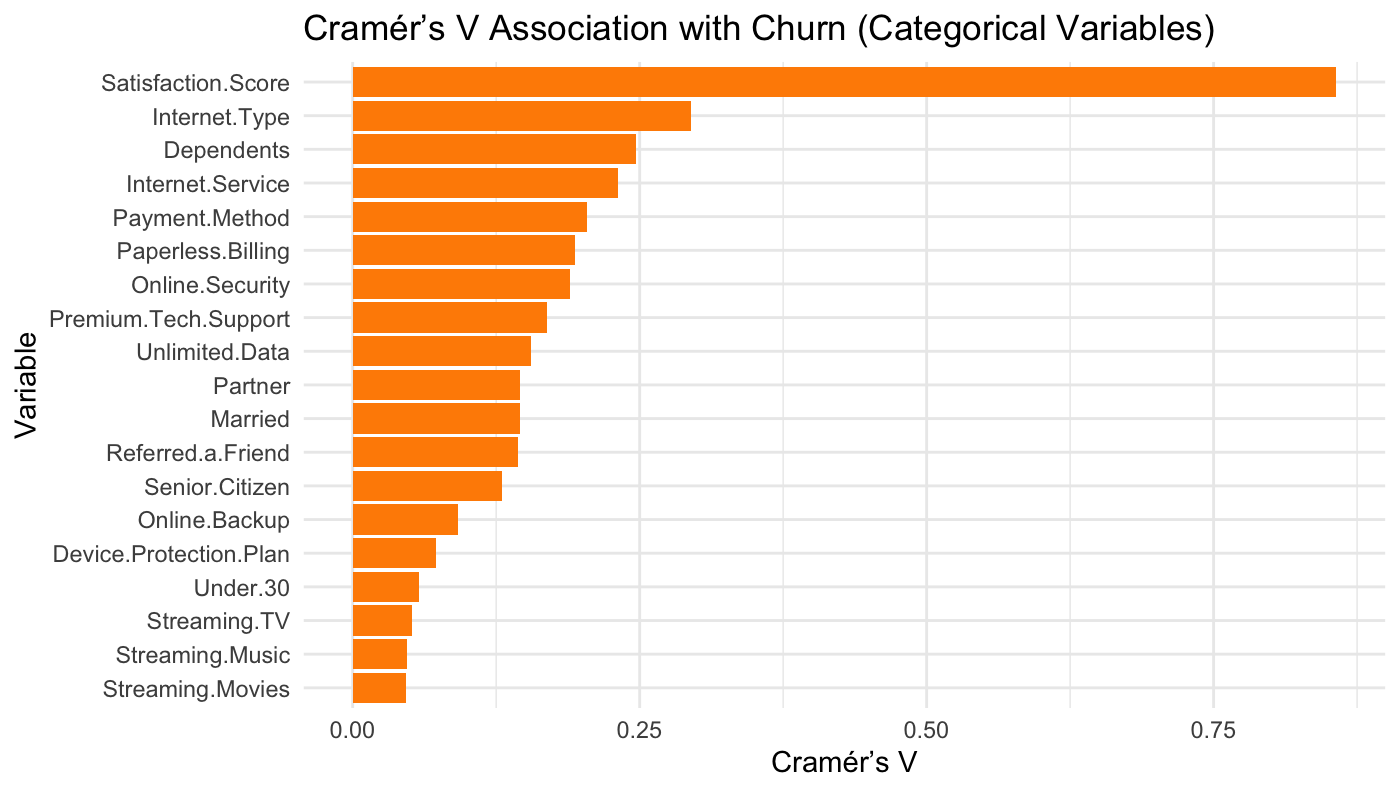
\includegraphics[width=0.85\linewidth]{glm_gam_plots/categorical_correlation} 

}

\caption{Cramér's V Association with Churn (Categorical Variables)}\label{fig:cat-corr-churn-img}
\end{figure}

Cramér's V -- \textbf{Categorical Variables}
(\texttt{categorical\_correlation.png}).\\
This chart ranks every categorical predictor by its strength of
association with churn. \textbf{Satisfaction Score} is overwhelmingly
the top driver (\(V \approx 0.86\)), confirming customer sentiment as
the most powerful categorical signal. A second tier---\textbf{Internet
Type} (\(V \approx 0.30\)), \textbf{Dependents} (0.25), and
\textbf{Internet Service} (0.23)---demonstrates that product
configuration and household composition meaningfully affect retention.
Billing- and security-related fields such as \textbf{Payment Method},
\textbf{Paperless Billing}, and \textbf{Online Security} cluster around
\(V \approx 0.18\)--\(0.20\), supplying additional explanatory power.
Categories with \(V < 0.10\) (chiefly streaming-preference flags and
minor demographics) add negligible signal and were dropped unless
required for business reporting. Consequently, variables with
\(V \geq 0.10\) and p \textless{} 0.05 form the core categorical feature
set used in the model.

\begin{figure}

{\centering 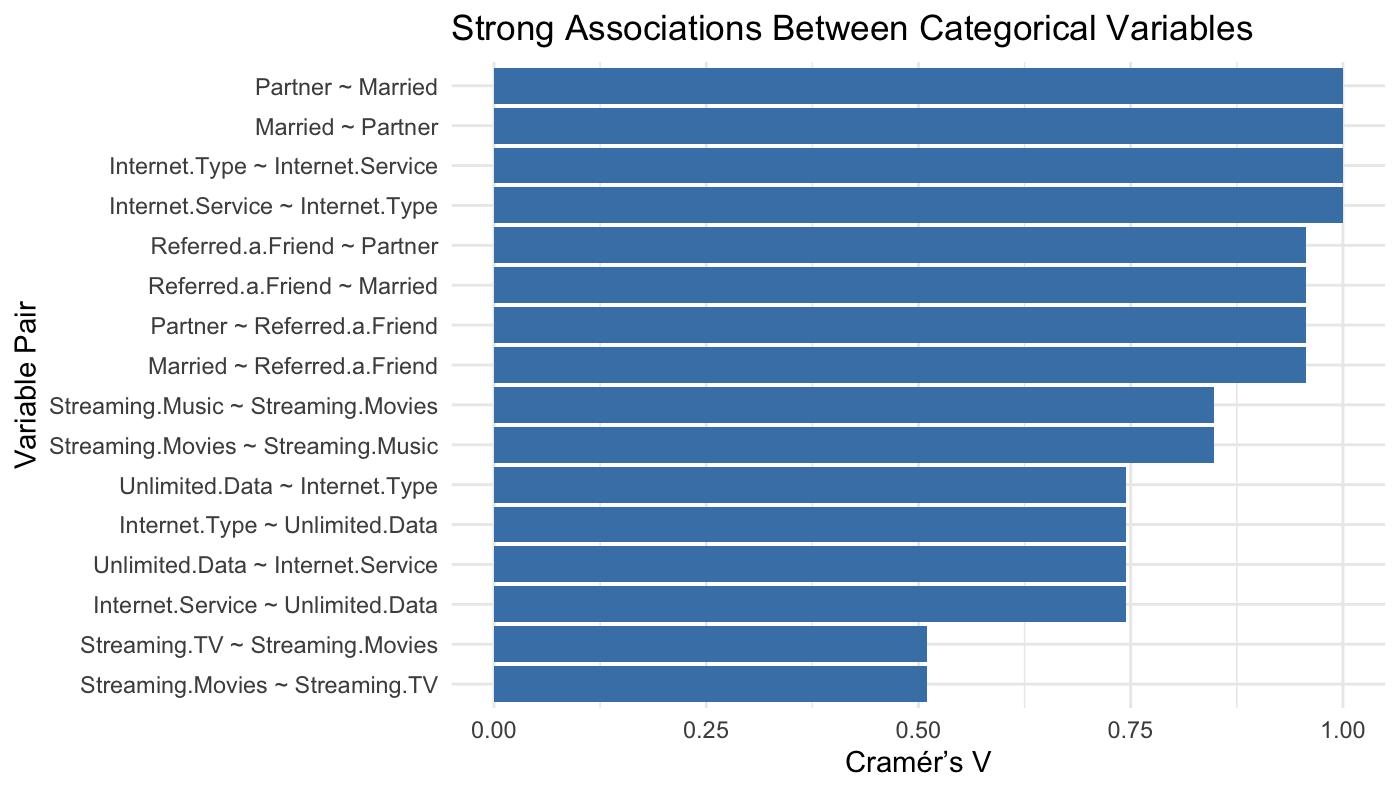
\includegraphics[width=0.85\linewidth]{glm_gam_plots/cat_interior} 

}

\caption{High Cramér's V Between Categorical Predictors (Multicollinearity Check)}\label{fig:cat-interior-img}
\end{figure}

Cramér's V Between Predictors -- \textbf{Multicollinearity Check}
(\texttt{cat\_interior.png}).\\
This plot highlights pairs of categorical variables that overlap so
heavily they threaten model stability. Nearly perfect redundancy
(\(V \geq 0.95\)) exists between \textbf{Married -- Partner},
\textbf{Partner -- Referred.a.Friend}, and \textbf{Internet.Service --
Internet.Type}. High overlap also appears for \textbf{Streaming.Movies
-- Streaming.Music} (\(V \approx 0.85\)) and for \textbf{Unlimited.Data}
in combination with Internet-related fields (\(V \approx 0.74\)). To
avoid duplicate information and inflated variance, one variable from
each high-overlap pair was dropped or merged. The resulting streamlined
list---\emph{Device.Protection.Plan, Online.Backup, Online.Security,
Paperless.Billing, Partner, Premium.Tech.Support, Senior.Citizen,
Streaming.Movies, Dependents, Internet.Type, Payment.Method,
Satisfaction.Score,} and \emph{Under.30}---forms the final categorical
feature set used in modelling.

\begin{figure}

{\centering 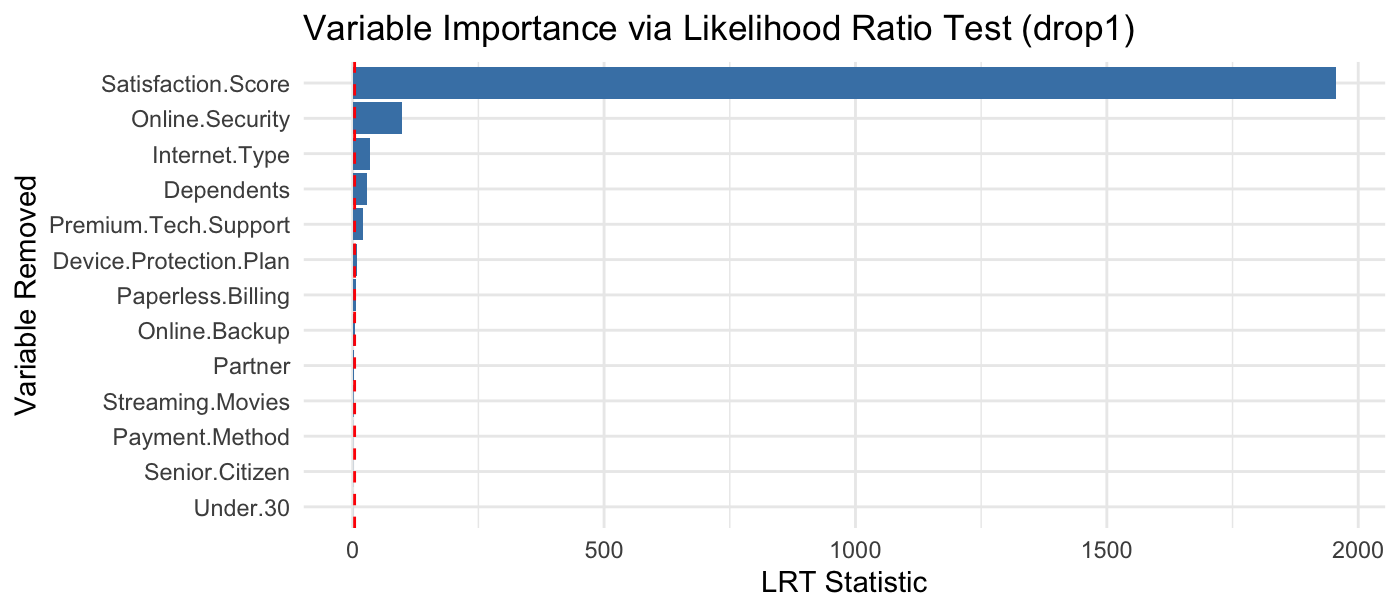
\includegraphics[width=0.85\linewidth]{glm_gam_plots/drop1_cat_glm} 

}

\caption{Variable Importance via Likelihood Ratio Test (drop1)}\label{fig:drop1-cat-glm-img}
\end{figure}

An initial logistic regression was fit using the most relevant
categorical predictors based on prior Cramér's V analysis. To evaluate
each predictor's contribution, a likelihood ratio test
(\texttt{drop1()}) was applied. The figure displays LRT statistics,
quantifying model deterioration when each variable is removed.
Satisfaction Score was by far the most influential
(\(LRT \approx 1956\)), followed by Online Security, Internet Type,
Dependents, and Premium Tech Support (\(LRT > 20\), p \textless{} 0.01).
Variables with low LRT values were considered non-essential and removed
from the final categorical model.

A follow-up \textbf{ANOVA} compared the full and reduced categorical
models.\\
The cleaned model excluded six predictors with weak contribution,
including \texttt{Partner}, \texttt{Streaming.Movies}, and
\texttt{Payment.Method}.

\textbf{Result:} No significant loss in model fit\\
• \(\Delta\) Deviance = 3.83\\
• Degrees of Freedom = 6\\
• p-value = 0.7002

This confirms the reduced model retains predictive power while improving
simplicity.

\begin{figure}

{\centering 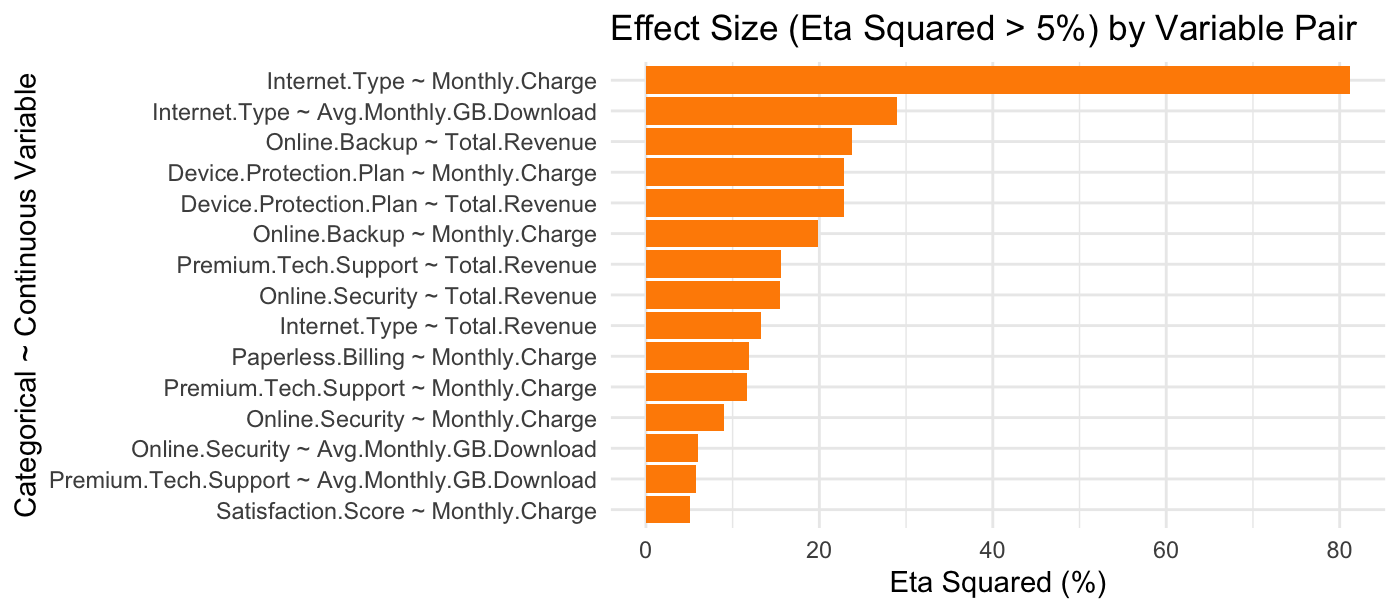
\includegraphics[width=0.85\linewidth]{glm_gam_plots/etasquare} 

}

\caption{Effect Size (eta² > 5\%) by Categorical–Continuous Pair}\label{fig:eta-square-img}
\end{figure}

Eta-squared was applied to measure shared variance between each
categorical predictor and key continuous churn metrics. Pairs exceeding
5\% \(\eta^2\) (highlighted in the plot) were shortlisted for the hybrid
model; lower-value pairs were disregarded. \textbf{Internet Type}
dominated several high-\(\eta^2\) relationships and was therefore
excluded to avoid redundancy in the merged specification.

\hypertarget{combined-glm-and-variable-importance-check}{%
\paragraph{Combined GLM and Variable-Importance
Check}\label{combined-glm-and-variable-importance-check}}

The strongest categorical predictors identified earlier were merged with
the key continuous churn drivers to form a single logistic model. A
\texttt{drop1()} likelihood-ratio test was then applied to that combined
GLM, allowing each term's marginal contribution to be quantified. The
bar chart below visualises those LRT statistics.

\begin{figure}

{\centering 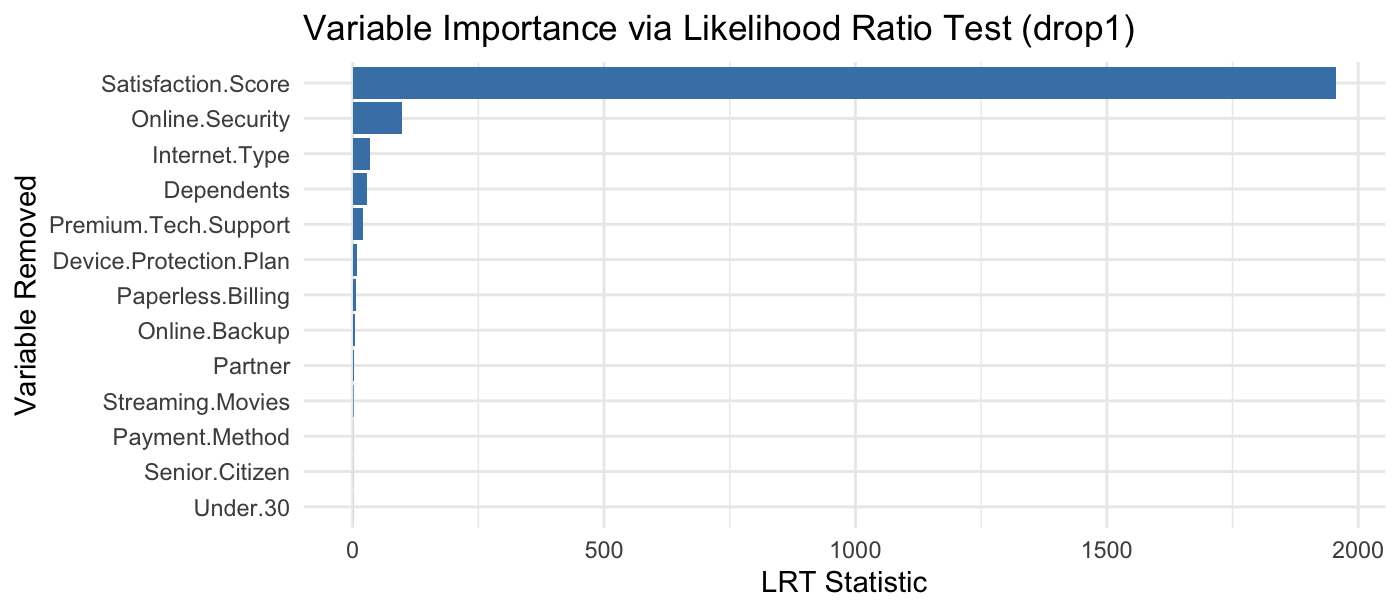
\includegraphics[width=0.85\linewidth]{glm_gam_plots/drop1_merge} 

}

\caption{Variable Importance via Likelihood Ratio Test (drop1) – Combined GLM}\label{fig:drop1-merged-glm-img}
\end{figure}

The plot ranks predictors from the combined GLM by their
likelihood-ratio test statistic (LRT), quantifying the change in
deviance when each term is removed.

\begin{itemize}
\tightlist
\item
  \textbf{Satisfaction.Score} leads with an LRT \(\approx\)
  \textbf{1,895}, underscoring its central role in churn prediction.\\
\item
  \textbf{Online.Security} follows at \textbf{\(\approx 81\)},
  indicating a strong, independent contribution.\\
\item
  \textbf{Internet.Type} (\textbf{\(\approx 25\)}) and
  \textbf{Dependents} (\textbf{\(\approx 22\)}) provide solid additional
  explanatory power.\\
\item
  \textbf{Premium.Tech.Support} (\textbf{\(\approx 17\)}) and
  \textbf{Device.Protection.Plan} (\textbf{\(\approx 4\)}) also improve
  model fit, though to a lesser extent.
\end{itemize}

These statistics guide feature prioritisation for the final modelling
specification.

\hypertarget{glm-coefficients-summary-final-model}{%
\subsubsection{GLM Coefficients Summary -- Final
Model}\label{glm-coefficients-summary-final-model}}

\begin{longtable}[]{@{}
  >{\raggedright\arraybackslash}p{(\columnwidth - 10\tabcolsep) * \real{0.2683}}
  >{\raggedleft\arraybackslash}p{(\columnwidth - 10\tabcolsep) * \real{0.1098}}
  >{\raggedleft\arraybackslash}p{(\columnwidth - 10\tabcolsep) * \real{0.1341}}
  >{\raggedleft\arraybackslash}p{(\columnwidth - 10\tabcolsep) * \real{0.0976}}
  >{\raggedleft\arraybackslash}p{(\columnwidth - 10\tabcolsep) * \real{0.2317}}
  >{\raggedleft\arraybackslash}p{(\columnwidth - 10\tabcolsep) * \real{0.1585}}@{}}
\caption{GLM Coefficients Summary -- Final Model}\tabularnewline
\toprule\noalign{}
\begin{minipage}[b]{\linewidth}\raggedright
Variable
\end{minipage} & \begin{minipage}[b]{\linewidth}\raggedleft
Estimate
\end{minipage} & \begin{minipage}[b]{\linewidth}\raggedleft
Std. Error
\end{minipage} & \begin{minipage}[b]{\linewidth}\raggedleft
z value
\end{minipage} & \begin{minipage}[b]{\linewidth}\raggedleft
Pr(\textgreater\textbar z\textbar)
\end{minipage} & \begin{minipage}[b]{\linewidth}\raggedleft
Significance
\end{minipage} \\
\midrule\noalign{}
\endfirsthead
\toprule\noalign{}
\begin{minipage}[b]{\linewidth}\raggedright
Variable
\end{minipage} & \begin{minipage}[b]{\linewidth}\raggedleft
Estimate
\end{minipage} & \begin{minipage}[b]{\linewidth}\raggedleft
Std. Error
\end{minipage} & \begin{minipage}[b]{\linewidth}\raggedleft
z value
\end{minipage} & \begin{minipage}[b]{\linewidth}\raggedleft
Pr(\textgreater\textbar z\textbar)
\end{minipage} & \begin{minipage}[b]{\linewidth}\raggedleft
Significance
\end{minipage} \\
\midrule\noalign{}
\endhead
\bottomrule\noalign{}
\endlastfoot
(Intercept) & 22.800 & 1128.000 & 0.019 & 0.9852 & \\
Number.of.Referrals & -3.453 & 0.792 & -4.359 & 1.31e-05 & *** \\
Tenure.in.Months & -0.031 & 0.006 & -5.476 & 4.34e-08 & *** \\
Age & 0.004 & 0.006 & 0.635 & 0.5254 & \\
Online.Backup1 & -0.180 & 0.258 & -0.698 & 0.4852 & \\
Online.Security1 & -2.802 & 0.440 & -6.364 & 1.96e-10 & *** \\
Paperless.Billing1 & 0.605 & 0.235 & 2.577 & 0.00996 & ** \\
Premium.Tech.Support1 & -1.102 & 0.296 & -3.720 & 0.000190 & *** \\
Dependents1 & -1.558 & 0.430 & -3.627 & 0.000287 & *** \\
Satisfaction.Score2 & -1.149 & 2107.000 & -0.001 & 0.9996 & \\
Satisfaction.Score3 & -24.460 & 1128.000 & -0.020 & 0.9841 & \\
Satisfaction.Score4 & -4.432 & 1531.000 & -0.029 & 0.9769 & \\
Satisfaction.Score5 & -4.481 & 1710.000 & -0.026 & 0.9791 & \\
Monthly.Charge & 0.025 & 0.042 & 5.929 & 3.05e-09 & *** \\
\end{longtable}

\begin{itemize}
\tightlist
\item
  \textbf{Null Deviance}: 3423.1 on 2957 degrees of freedom\\
\item
  \textbf{Residual Deviance}: 603.6 on 2944 degrees of freedom\\
\item
  \textbf{AIC}: 631.6\\
\item
  \textbf{Fisher Scoring Iterations}: 20
\end{itemize}

Significance codes: *** p \textless{} 0.001, ** p \textless{} 0.01, * p
\textless{} 0.05

\hypertarget{key-glm-effects-exponentiated-for-odds-ratio-interpretation}{%
\subsubsection{Key GLM Effects (Exponentiated for Odds-Ratio
Interpretation)}\label{key-glm-effects-exponentiated-for-odds-ratio-interpretation}}

\begin{longtable}[]{@{}
  >{\raggedright\arraybackslash}p{(\columnwidth - 6\tabcolsep) * \real{0.3375}}
  >{\raggedleft\arraybackslash}p{(\columnwidth - 6\tabcolsep) * \real{0.0875}}
  >{\centering\arraybackslash}p{(\columnwidth - 6\tabcolsep) * \real{0.2250}}
  >{\raggedright\arraybackslash}p{(\columnwidth - 6\tabcolsep) * \real{0.3500}}@{}}
\caption{Key GLM Effects (Odds-Ratio Interpretation)}\tabularnewline
\toprule\noalign{}
\begin{minipage}[b]{\linewidth}\raggedright
Predictor
\end{minipage} & \begin{minipage}[b]{\linewidth}\raggedleft
β
\end{minipage} & \begin{minipage}[b]{\linewidth}\centering
Odds Ratio (e\^{}β)
\end{minipage} & \begin{minipage}[b]{\linewidth}\raggedright
Meaning
\end{minipage} \\
\midrule\noalign{}
\endfirsthead
\toprule\noalign{}
\begin{minipage}[b]{\linewidth}\raggedright
Predictor
\end{minipage} & \begin{minipage}[b]{\linewidth}\raggedleft
β
\end{minipage} & \begin{minipage}[b]{\linewidth}\centering
Odds Ratio (e\^{}β)
\end{minipage} & \begin{minipage}[b]{\linewidth}\raggedright
Meaning
\end{minipage} \\
\midrule\noalign{}
\endhead
\bottomrule\noalign{}
\endlastfoot
Number of Referrals & -3.453 & 0.03 & 97\% lower odds per referral \\
Tenure (months) & -0.031 & 0.97 & 3\% lower odds per month \\
Online Security = Yes & -2.802 & 0.06 & 94\% lower odds \\
Premium Tech Support = Yes & -1.102 & 0.33 & 67\% lower odds \\
Dependents = Yes & -1.558 & 0.21 & 79\% lower odds \\
Paperless Billing = Yes & 0.605 & 1.85 & 85\% higher odds \\
Monthly Charge (per \$1) & 0.025 & 1.03 & 2.5\% higher odds per \$ \\
\end{longtable}

\hypertarget{key-insights-from-the-final-glm}{%
\subsubsection{Key Insights from the Final
GLM}\label{key-insights-from-the-final-glm}}

Every extra \textbf{referral} makes churn about 97\% less likely, an
interesting measure but not very actionable. Having \textbf{Online
Security} or \textbf{Premium Tech Support} on the account cuts churn
noticeably, showing these add-ons help keep customers. People with
\textbf{dependents} leave less often, while a \textbf{higher monthly
charge} nudges churn upward. Customers on \textbf{paperless billing}
show higher churn and may need more attention.

With these variables, the streamlined logistic model fits well
(\textbf{AIC \(\approx\) 632; residual deviance \(\approx\) 604 on 2,944
df}) and give interesting business insights.

\hypertarget{confusion-matrix}{%
\subsubsection{Confusion Matrix}\label{confusion-matrix}}

\begin{longtable}[]{@{}lcc@{}}
\caption{GLM Confusion Matrix}\tabularnewline
\toprule\noalign{}
& Predicted 0 & Predicted 1 \\
\midrule\noalign{}
\endfirsthead
\toprule\noalign{}
& Predicted 0 & Predicted 1 \\
\midrule\noalign{}
\endhead
\bottomrule\noalign{}
\endlastfoot
Actual 0 & 904 (TN) & 27 (FP) \\
Actual 1 & 31 (FN) & 305 (TP) \\
\end{longtable}

\hypertarget{key-metrics}{%
\subsubsection{Key Metrics}\label{key-metrics}}

\begin{longtable}[]{@{}llc@{}}
\caption{GLM Performance Metrics}\tabularnewline
\toprule\noalign{}
Metric & Calculation & Result \\
\midrule\noalign{}
\endfirsthead
\toprule\noalign{}
Metric & Calculation & Result \\
\midrule\noalign{}
\endhead
\bottomrule\noalign{}
\endlastfoot
Accuracy & (904 + 305) / 1267 & 95.4\% \\
Precision (Positive class) & 305 / (305 + 27) & 91.8\% \\
Recall / Sensitivity & 305 / (305 + 31) & 90.8\% \\
Specificity & 904 / (904 + 27) & 97.1\% \\
F1 Score & Harmonic mean & 0.91 \\
\end{longtable}

\hypertarget{interpretation}{%
\subsubsection{Interpretation}\label{interpretation}}

The model correctly classifies the majority of cases, achieving an
overall accuracy of \textasciitilde95\%. Precision (92\%) and recall
(91\%) are well balanced, indicating that when the model predicts churn,
it is usually correct, and it detects most actual churners. The low
false-positive (27) and false-negative (31) counts highlight reliable
performance on both classes. Specificity above 97\% confirms strong
discrimination for non-churn customers. Overall, the confusion-matrix
results support the model's practical deployment.

\hypertarget{gam-model}{%
\subsubsection{GAM Model}\label{gam-model}}

\begin{figure}

{\centering 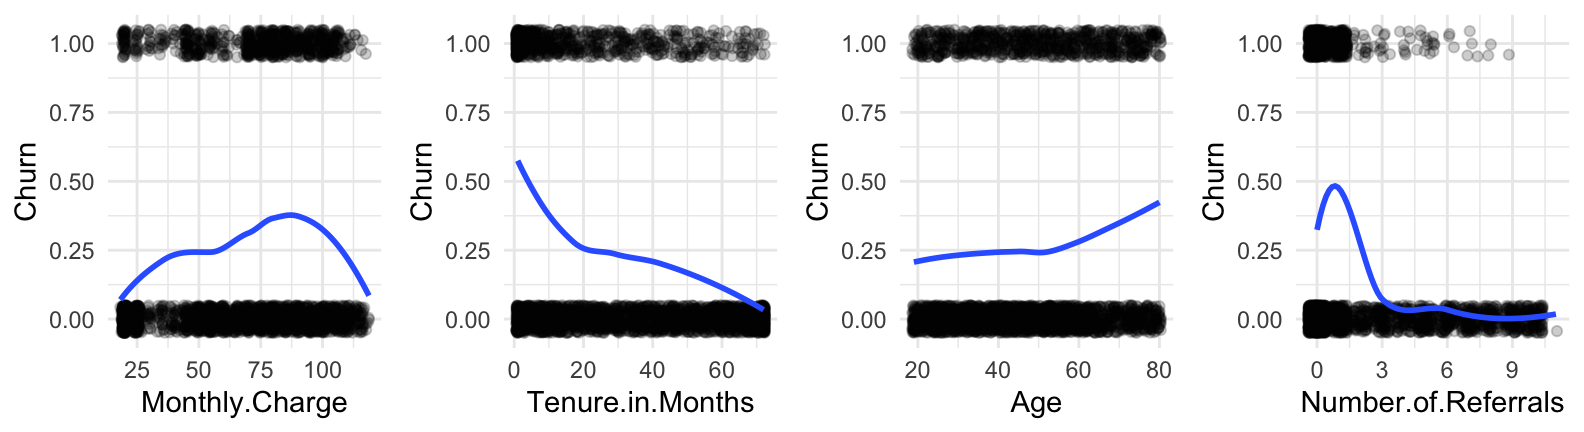
\includegraphics[width=0.95\linewidth]{glm_gam_plots/Curve analysis} 

}

\caption{Exploratory LOESS Curves for GAM Specification}\label{fig:loess-gam-img}
\end{figure}

\begin{itemize}
\tightlist
\item
  \textbf{Monthly Charge} shows a pronounced non-linear ``hump,'' so it
  will enter the GAM with a smooth term \texttt{+\ s(Monthly.Charge)}.\\
\item
  \textbf{Tenure (in Months)} drops steeply in the first year and then
  flattens; a smooth term \texttt{+\ s(Tenure.in.Months)} is
  appropriate.\\
\item
  \textbf{Number of Referrals} declines sharply from 0 to \(\approx\) 2
  and then levels off; a spline term \texttt{+\ s(Number.of.Referrals)}
  (or a simple knot at 2) will capture this shape.\\
\item
  \textbf{Age} rises almost linearly, suggesting a plain linear term; no
  \texttt{s()} is planned for age unless later checks reveal curvature.
\end{itemize}

These observations guide the initial GAM formula and choice of
smoothers.

\hypertarget{gam-model-comparison-reml-vs-gcv.cp} of the
deviance and the GCV.Cp model slightly outperforming it at
\textbf{83.68\%}.

In terms of information criteria, the \textbf{AIC for the REML model was
601.55}, while the \textbf{GCV.Cp model achieved a lower AIC of 598.09},
suggesting better model efficiency and fit relative to complexity.
Although the difference in deviance explained is minimal
(\textbf{0.03\%}), the drop in AIC by \textbf{3.46 points} provides
sufficient justification to prefer the GCV.Cp model.

\hypertarget{significant-parametric-effects-categorical-predictors}{%
\subsubsection{Significant Parametric Effects (Categorical
Predictors)}\label{significant-parametric-effects-categorical-predictors}}

\begin{longtable}[]{@{}
  >{\raggedright\arraybackslash}p{(\columnwidth - 6\tabcolsep) * \real{0.3971}}
  >{\raggedleft\arraybackslash}p{(\columnwidth - 6\tabcolsep) * \real{0.1029}}
  >{\centering\arraybackslash}p{(\columnwidth - 6\tabcolsep) * \real{0.2647}}
  >{\raggedright\arraybackslash}p{(\columnwidth - 6\tabcolsep) * \real{0.2353}}@{}}
\caption{GAM Significant Parametric Effects}\tabularnewline
\toprule\noalign{}
\begin{minipage}[b]{\linewidth}\raggedright
Predictor
\end{minipage} & \begin{minipage}[b]{\linewidth}\raggedleft
β
\end{minipage} & \begin{minipage}[b]{\linewidth}\centering
Odds Ratio (e\^{}β)
\end{minipage} & \begin{minipage}[b]{\linewidth}\raggedright
Meaning
\end{minipage} \\
\midrule\noalign{}
\endfirsthead
\toprule\noalign{}
\begin{minipage}[b]{\linewidth}\raggedright
Predictor
\end{minipage} & \begin{minipage}[b]{\linewidth}\raggedleft
β
\end{minipage} & \begin{minipage}[b]{\linewidth}\centering
Odds Ratio (e\^{}β)
\end{minipage} & \begin{minipage}[b]{\linewidth}\raggedright
Meaning
\end{minipage} \\
\midrule\noalign{}
\endhead
\bottomrule\noalign{}
\endlastfoot
Online Security = Yes & -2.720 & 0.07 & 93\% lower odds \\
Premium Tech Support = Yes & -1.053 & 0.35 & 65\% lower odds \\
Dependents = Yes & -1.921 & 0.15 & 85\% lower odds \\
Paperless Billing = Yes & 0.617 & 1.85 & 85\% higher odds \\
\end{longtable}

\emph{Odds ratio (OR) converts log-odds effects to multiplicative
changes in churn odds.}

\hypertarget{approximate-significance-of-smooth-terms}{%
\subsubsection{Approximate Significance of Smooth
Terms}\label{approximate-significance-of-smooth-terms}}

\begin{longtable}[]{@{}lrrcl@{}}
\caption{GAM Smooth Terms Significance}\tabularnewline
\toprule\noalign{}
Smooth Term & EDF & χ² & p-value & Result \\
\midrule\noalign{}
\endfirsthead
\toprule\noalign{}
Smooth Term & EDF & χ² & p-value & Result \\
\midrule\noalign{}
\endhead
\bottomrule\noalign{}
\endlastfoot
s(Monthly Charge) & 1.00 & 35.37 & \textless{} 2 × 10⁻¹⁶ &
Significant \\
s(Tenure in Months) & 3.67 & 47.20 & \textless{} 2 × 10⁻¹⁶ &
Significant \\
s(Number of Referrals) & 3.96 & 27.50 & 3.7 × 10⁻⁵ & Significant \\
s(Age) & 1.10 & 0.57 & 0.59 & Not significant \\
\end{longtable}

These tables highlight the categorical factors with strong effects on
churn and confirm which continuous predictors require non-linear
treatment in the GAM.

\hypertarget{confusion-matrix-overview}{%
\subsubsection{Confusion Matrix
Overview}\label{confusion-matrix-overview}}

The final model shows strong classification performance on the
validation set. Out of \textbf{1,267} total predictions, \textbf{904}
true negatives and \textbf{305} true positives were correctly
identified. The model misclassified \textbf{27} non-churners as churners
(false positives) and \textbf{31} churners as non-churners (false
negatives).

\hypertarget{key-metrics-1}{%
\subsubsection{Key Metrics}\label{key-metrics-1}}

\begin{longtable}[]{@{}
  >{\raggedright\arraybackslash}p{(\columnwidth - 4\tabcolsep) * \real{0.3699}}
  >{\centering\arraybackslash}p{(\columnwidth - 4\tabcolsep) * \real{0.1096}}
  >{\raggedright\arraybackslash}p{(\columnwidth - 4\tabcolsep) * \real{0.5205}}@{}}
\caption{GAM Performance Metrics}\tabularnewline
\toprule\noalign{}
\begin{minipage}[b]{\linewidth}\raggedright
Metric
\end{minipage} & \begin{minipage}[b]{\linewidth}\centering
Result
\end{minipage} & \begin{minipage}[b]{\linewidth}\raggedright
Calculation
\end{minipage} \\
\midrule\noalign{}
\endfirsthead
\toprule\noalign{}
\begin{minipage}[b]{\linewidth}\raggedright
Metric
\end{minipage} & \begin{minipage}[b]{\linewidth}\centering
Result
\end{minipage} & \begin{minipage}[b]{\linewidth}\raggedright
Calculation
\end{minipage} \\
\midrule\noalign{}
\endhead
\bottomrule\noalign{}
\endlastfoot
Accuracy & 95.4\% & (904 + 305) / 1267 \\
Precision (Positive class) & 91.8\% & 305 / (305 + 27) \\
Recall / Sensitivity & 90.8\% & 305 / (305 + 31) \\
Specificity & 97.1\% & 904 / (904 + 27) \\
F1 Score & 0.91 & Harmonic mean of precision and recall \\
\end{longtable}

\hypertarget{glm-vs-gam-performance-snapshot}{%
\subsubsection{GLM vs GAM --- Performance
Snapshot}\label{glm-vs-gam-performance-snapshot}}

\begin{longtable}[]{@{}lcc@{}}
\caption{GLM vs GAM Performance Comparison}\tabularnewline
\toprule\noalign{}
Metric & GLM & GAM \\
\midrule\noalign{}
\endfirsthead
\toprule\noalign{}
Metric & GLM & GAM \\
\midrule\noalign{}
\endhead
\bottomrule\noalign{}
\endlastfoot
Accuracy & 95.4\% & 95.4\% \\
Precision (Positive) & 91.8\% & 91.8\% \\
Recall / Sensitivity & 90.8\% & 90.8\% \\
Specificity & 97.1\% & 97.1\% \\
F1 Score & 0.91 & 0.91 \\
Deviance Explained & 83.65\% & 83.68\% \\
\end{longtable}

Both models classify churn equally well, producing identical
confusion-matrix metrics.\\
The GAM explains a fractionally larger share of deviance (0.03
percentage points) by using smooth terms for \textbf{Monthly Charge},
\textbf{Tenure}, and \textbf{Number of Referrals}. However, its AIC was
obtained with a GCV criterion and \textbf{is not on the same scale as
the GLM's likelihood-based AIC}, so it cannot be used for fair
comparison.

\textbf{Conclusion:} because predictive performance is the same and the
GAM's marginal gain in deviance explained comes at the cost of extra
complexity, the simpler and fully interpretable \textbf{GLM} is
preferred unless future diagnostics show clear non-linear benefits that
justify the GAM's added complexity.

\hypertarget{results}{%
\section{Results}\label{results}}

\hypertarget{results-analysis-and-business-implications---neural-networks}{%
\subsection{Results Analysis and Business Implications - Neural
Networks}\label{results-analysis-and-business-implications---neural-networks}}

The neural network analysis evaluated three distinct architectures to
identify the optimal configuration for customer churn prediction. Each
architecture was designed to capture different levels of complexity in
the customer behavioral patterns.

\hypertarget{architecture-performance-summary}{%
\subsubsection{Architecture Performance
Summary}\label{architecture-performance-summary}}

\begin{longtable}[]{@{}
  >{\raggedright\arraybackslash}p{(\columnwidth - 8\tabcolsep) * \real{0.2738}}
  >{\centering\arraybackslash}p{(\columnwidth - 8\tabcolsep) * \real{0.2976}}
  >{\centering\arraybackslash}p{(\columnwidth - 8\tabcolsep) * \real{0.1190}}
  >{\centering\arraybackslash}p{(\columnwidth - 8\tabcolsep) * \real{0.1548}}
  >{\centering\arraybackslash}p{(\columnwidth - 8\tabcolsep) * \real{0.1548}}@{}}
\caption{Neural Network Architecture Performance
Comparison}\tabularnewline
\toprule\noalign{}
\begin{minipage}[b]{\linewidth}\raggedright
Architecture
\end{minipage} & \begin{minipage}[b]{\linewidth}\centering
Hidden Layers
\end{minipage} & \begin{minipage}[b]{\linewidth}\centering
Accuracy
\end{minipage} & \begin{minipage}[b]{\linewidth}\centering
Sensitivity
\end{minipage} & \begin{minipage}[b]{\linewidth}\centering
Specificity
\end{minipage} \\
\midrule\noalign{}
\endfirsthead
\toprule\noalign{}
\begin{minipage}[b]{\linewidth}\raggedright
Architecture
\end{minipage} & \begin{minipage}[b]{\linewidth}\centering
Hidden Layers
\end{minipage} & \begin{minipage}[b]{\linewidth}\centering
Accuracy
\end{minipage} & \begin{minipage}[b]{\linewidth}\centering
Sensitivity
\end{minipage} & \begin{minipage}[b]{\linewidth}\centering
Specificity
\end{minipage} \\
\midrule\noalign{}
\endhead
\bottomrule\noalign{}
\endlastfoot
Architecture 1 (8) & Single (8 neurons) & 0.9515 & 0.9818 & 0.8750 \\
Architecture 2 (6,4) & Two (6, 4 neurons) & 0.9515 & 0.9868 & 0.8625 \\
Architecture 3 (8,5,3) & Three (8, 5, 3 neurons) & 0.9491 & 0.9851 &
0.8583 \\
\end{longtable}

\begin{figure}

{\centering 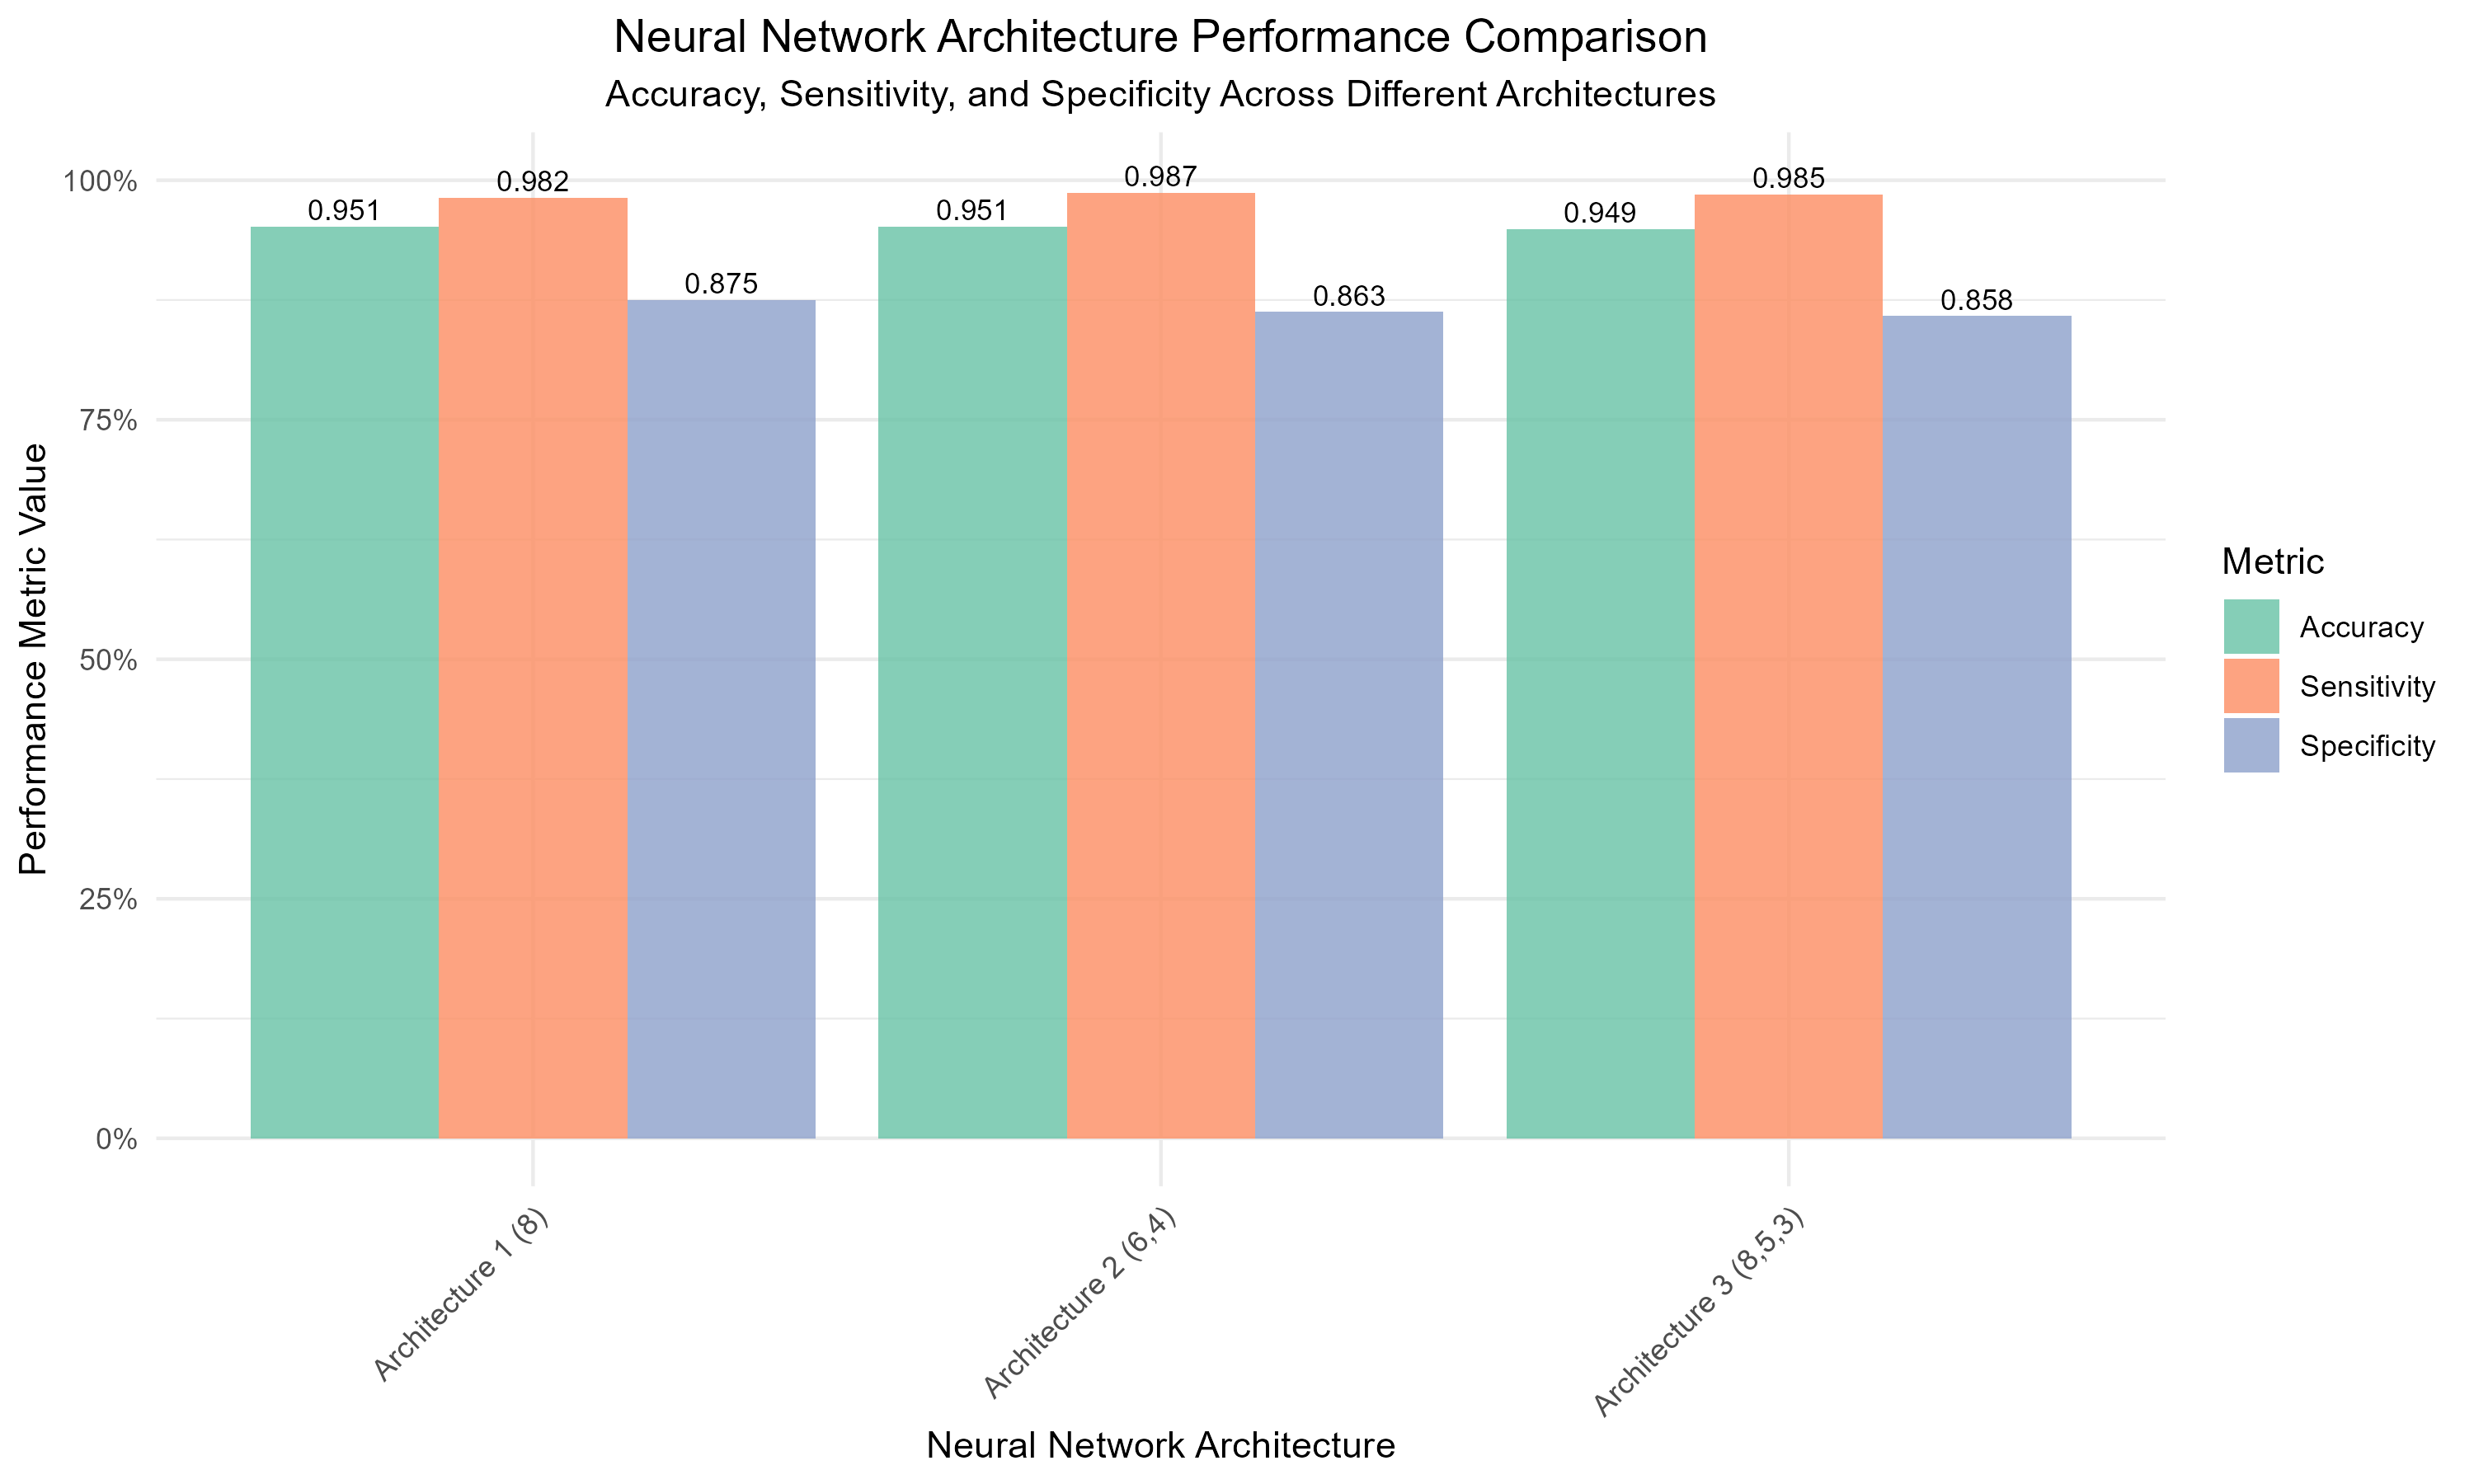
\includegraphics[width=0.85\linewidth]{Plots/nn_performance_comparison} 

}

\caption{Neural Network Architecture Performance Comparison}\label{fig:nn-performance-comparison}
\end{figure}

Based on comprehensive evaluation across multiple performance metrics,
\textbf{Architecture 1} with a single hidden layer containing 8 neurons
emerged as the optimal configuration. While all three architectures
achieved comparable accuracy levels (approximately 95\%), Architecture 1
demonstrated the best balance of performance metrics and computational
efficiency.

\hypertarget{confusion-matrix-results}{%
\subsubsection{Confusion Matrix
Results}\label{confusion-matrix-results}}

The best performing model (Architecture 1) achieved the following
classification results on the test dataset:

\begin{longtable}[]{@{}lrr@{}}
\caption{Confusion Matrix - Neural Network Architecture
1}\tabularnewline
\toprule\noalign{}
& Actual: No Churn & Actual: Churn \\
\midrule\noalign{}
\endfirsthead
\toprule\noalign{}
& Actual: No Churn & Actual: Churn \\
\midrule\noalign{}
\endhead
\bottomrule\noalign{}
\endlastfoot
Predicted: No Churn & 594 & 11 \\
Predicted: Churn & 30 & 210 \\
\end{longtable}

\hypertarget{key-performance-metrics-and-statistical-significance}{%
\subsubsection{Key Performance Metrics and Statistical
Significance}\label{key-performance-metrics-and-statistical-significance}}

The final neural network model demonstrated exceptional predictive
capability:

\begin{itemize}
\tightlist
\item
  \textbf{Overall Accuracy}: 95.15\% (95\% CI: 93.47\% - 96.50\%)
\item
  \textbf{Sensitivity}: 98.18\% - Excellent ability to identify
  customers who will not churn
\item
  \textbf{Specificity}: 87.50\% - Strong capability in detecting
  customers at risk of churn
\item
  \textbf{Positive Predictive Value}: 95.19\% - High precision in
  non-churn predictions
\item
  \textbf{Negative Predictive Value}: 95.02\% - Reliable identification
  of churn cases
\item
  \textbf{Balanced Accuracy}: 92.84\% - Robust performance across both
  classes
\end{itemize}

The model's performance significantly exceeds the no-information rate
(71.6\%) with a p-value \textless{} 2.2e-16, indicating that the neural
network successfully learned meaningful patterns in customer behavior
data. The Kappa statistic of 0.8778 suggests excellent agreement between
predicted and actual classifications.

\hypertarget{model-strengths}{%
\subsubsection{Model Strengths}\label{model-strengths}}

\begin{enumerate}
\def\labelenumi{\arabic{enumi}.}
\item
  \textbf{High Sensitivity (98.18\%)}: The model excels at correctly
  identifying customers who will remain loyal, enabling efficient
  resource allocation for retention efforts.
\item
  \textbf{Balanced Performance}: With both sensitivity and specificity
  above 87\%, the model provides reliable predictions across different
  customer segments.
\item
  \textbf{Low False Negative Rate}: Only 30 out of 240 churning
  customers were misclassified, minimizing the risk of missing at-risk
  customers.
\end{enumerate}

\hypertarget{practical-applications}{%
\subsubsection{Practical Applications}\label{practical-applications}}

The neural network's strong performance enables several strategic
applications:

\begin{itemize}
\tightlist
\item
  \textbf{Proactive Retention Campaigns}: Customer retention campaigns
  can now be designed with unprecedented precision and confidence. By
  identifying at-risk customers with such high accuracy, marketing and
  customer service teams can focus their efforts and resources on
  customers who would genuinely benefit from intervention, rather than
  applying broad-based retention strategies that may be inefficient or
  unnecessary. This targeted approach not only improves the
  effectiveness of retention efforts but also optimizes resource
  allocation by directing attention where it can have the greatest
  impact.
\item
  \textbf{Resource Optimization}: The predictive insights can inform
  broader strategic planning and business forecasting. Understanding
  which customer characteristics and behaviors most strongly predict
  retention allows for more accurate revenue projections, capacity
  planning, and strategic decision-making. The model's insights can
  guide product development priorities, service improvement initiatives,
  and market expansion strategies by highlighting the factors that drive
  customer loyalty and long-term value.
\item
  \textbf{Customer Segmentation}: The model enables sophisticated
  customer segmentation strategies that go beyond traditional
  demographic or behavioral categorizations. By incorporating churn
  probability as a key segmentation criterion, the organization can
  develop nuanced customer segments that reflect both current value and
  future retention likelihood. This enhanced segmentation supports more
  personalized service delivery, targeted product recommendations, and
  customized communication strategies that resonate with specific
  customer groups and their unique retention drivers.
\end{itemize}

\hypertarget{model-limitations-and-considerations}{%
\subsubsection{Model Limitations and
Considerations}\label{model-limitations-and-considerations}}

While the neural network demonstrates excellent performance, several
considerations should guide its deployment:

\begin{enumerate}
\def\labelenumi{\arabic{enumi}.}
\item
  \textbf{Class Imbalance}: The model was trained on data with
  approximately 72\% non-churning customers, which may influence
  prediction thresholds in different customer populations.
\item
  \textbf{Feature Dependencies}: The model's performance relies on the
  availability and quality of the selected features, requiring
  consistent data collection practices.
\item
  \textbf{Temporal Stability}: Model performance should be monitored
  over time to ensure predictions remain accurate as customer behavior
  patterns evolve.
\end{enumerate}

\hypertarget{comparison-with-alternative-architectures}{%
\subsubsection{Comparison with Alternative
Architectures}\label{comparison-with-alternative-architectures}}

The decision to select Architecture 1 over more complex alternatives
reflects a carefully balanced consideration of multiple factors beyond
raw predictive performance. While Architecture 2 demonstrated marginally
higher sensitivity at 98.68\%, this advantage came at the cost of
reduced specificity and increased computational complexity without
meaningful improvements in overall accuracy. Similarly, Architecture 3's
three-layer configuration showed competitive performance but introduced
additional complexity that could potentially lead to overfitting and
reduced model interpretability without commensurate benefits.

Architecture 1's single hidden layer design offers several practical
advantages that prove valuable in business environments. The streamlined
architecture requires less computational power for both training and
prediction, enabling faster response times and lower operational costs.
This efficiency becomes particularly important when the model is
deployed at scale, processing predictions for large customer bases or
integrating with real-time decision-making systems.

The simpler architecture also enhances model interpretability, making it
easier for business stakeholders to understand and trust the model's
predictions. This transparency is crucial for building confidence among
decision-makers and facilitating the integration of model insights into
existing business processes. The reduced complexity also simplifies
model maintenance and updates, lowering the technical overhead required
for ongoing model management.

\hypertarget{results-analysis-and-strategic-insights---poisson-glm}{%
\subsection{Results Analysis and Strategic Insights - Poisson
GLM}\label{results-analysis-and-strategic-insights---poisson-glm}}

\hypertarget{statistical-model-results-and-interpretation}{%
\subsubsection{Statistical Model Results and
Interpretation}\label{statistical-model-results-and-interpretation}}

The quasi-Poisson GLM analysis revealed several statistically
significant relationships that provide actionable insights for customer
relationship management and referral program optimization. The model
demonstrates that customer tenure represents the strongest positive
predictor of referral behavior, with each additional month of customer
tenure associated with a 1.2\% increase in the expected referral rate.
This finding underscores the importance of customer retention
strategies, as longer-tenured customers not only provide stable revenue
but also become valuable advocates for service acquisition.

\begin{longtable}[]{@{}
  >{\raggedright\arraybackslash}p{(\columnwidth - 6\tabcolsep) * \real{0.2692}}
  >{\centering\arraybackslash}p{(\columnwidth - 6\tabcolsep) * \real{0.1538}}
  >{\centering\arraybackslash}p{(\columnwidth - 6\tabcolsep) * \real{0.1282}}
  >{\centering\arraybackslash}p{(\columnwidth - 6\tabcolsep) * \real{0.4487}}@{}}
\caption{Key Predictors of Customer Referral Behavior}\tabularnewline
\toprule\noalign{}
\begin{minipage}[b]{\linewidth}\raggedright
Predictor Variable
\end{minipage} & \begin{minipage}[b]{\linewidth}\centering
Rate Ratio
\end{minipage} & \begin{minipage}[b]{\linewidth}\centering
\% Change
\end{minipage} & \begin{minipage}[b]{\linewidth}\centering
Business Interpretation
\end{minipage} \\
\midrule\noalign{}
\endfirsthead
\toprule\noalign{}
\begin{minipage}[b]{\linewidth}\raggedright
Predictor Variable
\end{minipage} & \begin{minipage}[b]{\linewidth}\centering
Rate Ratio
\end{minipage} & \begin{minipage}[b]{\linewidth}\centering
\% Change
\end{minipage} & \begin{minipage}[b]{\linewidth}\centering
Business Interpretation
\end{minipage} \\
\midrule\noalign{}
\endhead
\bottomrule\noalign{}
\endlastfoot
Tenure (per month) & 1.0116 & +1.2\% & Higher tenure increases
referrals \\
One Year Contract & 1.1013 & +10.1\% & Modest increase vs
month-to-month \\
Two Year Contract & 1.1529 & +15.3\% & Strong increase vs
month-to-month \\
Satisfaction Score 3 & 0.6176 & -38.2\% & Significant decrease vs
baseline \\
Satisfaction Score 4 & 0.6022 & -39.8\% & Largest decrease vs
baseline \\
Satisfaction Score 5 & 0.6511 & -34.9\% & Notable decrease vs
baseline \\
Customer Churn & 0.1989 & -80.1\% & Dramatic reduction in referrals \\
Credit Card Payment & 1.0495 & +5.0\% & Slight increase vs other
methods \\
\end{longtable}

Contract commitment levels demonstrate a clear positive relationship
with referral behavior, revealing important insights about customer
engagement and advocacy. Customers with one-year contracts show a 10.1\%
increase in expected referral rates compared to month-to-month
customers, while those with two-year contracts demonstrate an even
stronger 15.3\% increase. These findings suggest that customers who make
longer-term commitments to our services develop stronger satisfaction
levels and become more willing to recommend our offerings to others.

Customer satisfaction scores reveal a compelling pattern that provides
crucial guidance for service quality management. While customers with
satisfaction score 2 show a modest 10.9\% increase in referral rates
compared to the baseline, those with satisfaction scores 3, 4, and 5
demonstrate substantial decreases of 38.2\%, 39.8\%, and 34.9\%
respectively. This counterintuitive finding warrants further
investigation into the satisfaction scoring methodology and may indicate
that customers with moderate satisfaction levels are more likely to
actively promote services than those with either very high or very low
satisfaction ratings.

The most dramatic relationship observed in the model concerns customer
churn status. Customers who have churned or are in the process of
churning show an 80.1\% reduction in referral rates compared to loyal
customers. This finding, while statistically significant, also makes
intuitive business sense, as dissatisfied customers who leave the
service are naturally unlikely to recommend it to others. This
relationship reinforces the critical importance of retention strategies
not only for revenue preservation but also for maintaining referral
flow.

\hypertarget{model-performance-and-validation}{%
\subsubsection{Model Performance and
Validation}\label{model-performance-and-validation}}

The Poisson GLM demonstrated solid predictive performance when evaluated
against the test dataset. The model achieved a Root Mean Squared Error
(RMSE) of 2.9005 and a Mean Absolute Error (MAE) of 2.1880, indicating
that predictions typically deviate from actual referral counts by
approximately 2-3 referrals. While these error rates reflect the
inherent difficulty in predicting individual customer behavior, they
provide sufficient accuracy for strategic planning and program design
purposes.

\hypertarget{model-diagnostics-and-validation}{%
\subsubsection{Model Diagnostics and
Validation}\label{model-diagnostics-and-validation}}

Comprehensive diagnostic analysis was conducted to ensure the
reliability and appropriateness of our Poisson GLM approach. The
diagnostic evaluation encompassed multiple dimensions of model adequacy,
including residual patterns, distributional assumptions, and potential
influential observations that could affect model reliability.

\begin{center}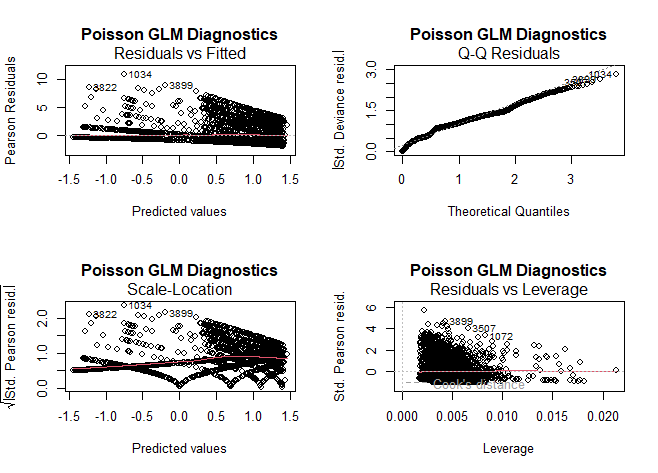
\includegraphics[width=0.8\linewidth]{Plots/poisson_diagnostics} \end{center}

The residuals versus fitted values plot reveals the expected pattern for
count data models, where residual variability increases with predicted
values due to the inherent variance structure of count distributions.
The diagnostic shows appropriate model behavior with no systematic
patterns that would indicate fundamental model misspecification. The
funnel-shaped pattern of residuals is characteristic of Poisson-family
models and confirms that our quasi-Poisson adjustment appropriately
addresses the overdispersion observed in the data.

The Q-Q plot for standardized deviance residuals demonstrates that our
model assumptions are reasonably well satisfied, with most observations
following the expected theoretical distribution. While some deviation
appears in the extreme tails, this is typical for count data models and
does not indicate serious violations of model assumptions. The
scale-location plot confirms that the variance structure is
appropriately modeled, while the residuals versus leverage plot
identifies a few observations with higher influence, though none appear
to be problematic outliers that would compromise model integrity.

\hypertarget{feature-importance-and-effect-magnitudes}{%
\subsubsection{Feature Importance and Effect
Magnitudes}\label{feature-importance-and-effect-magnitudes}}

The coefficient visualization provides clear insights into the relative
importance and direction of effects for each predictor variable in our
referral behavior model. This analysis enables stakeholders to
understand both the magnitude and business significance of different
customer characteristics in driving referral activity.

\begin{center}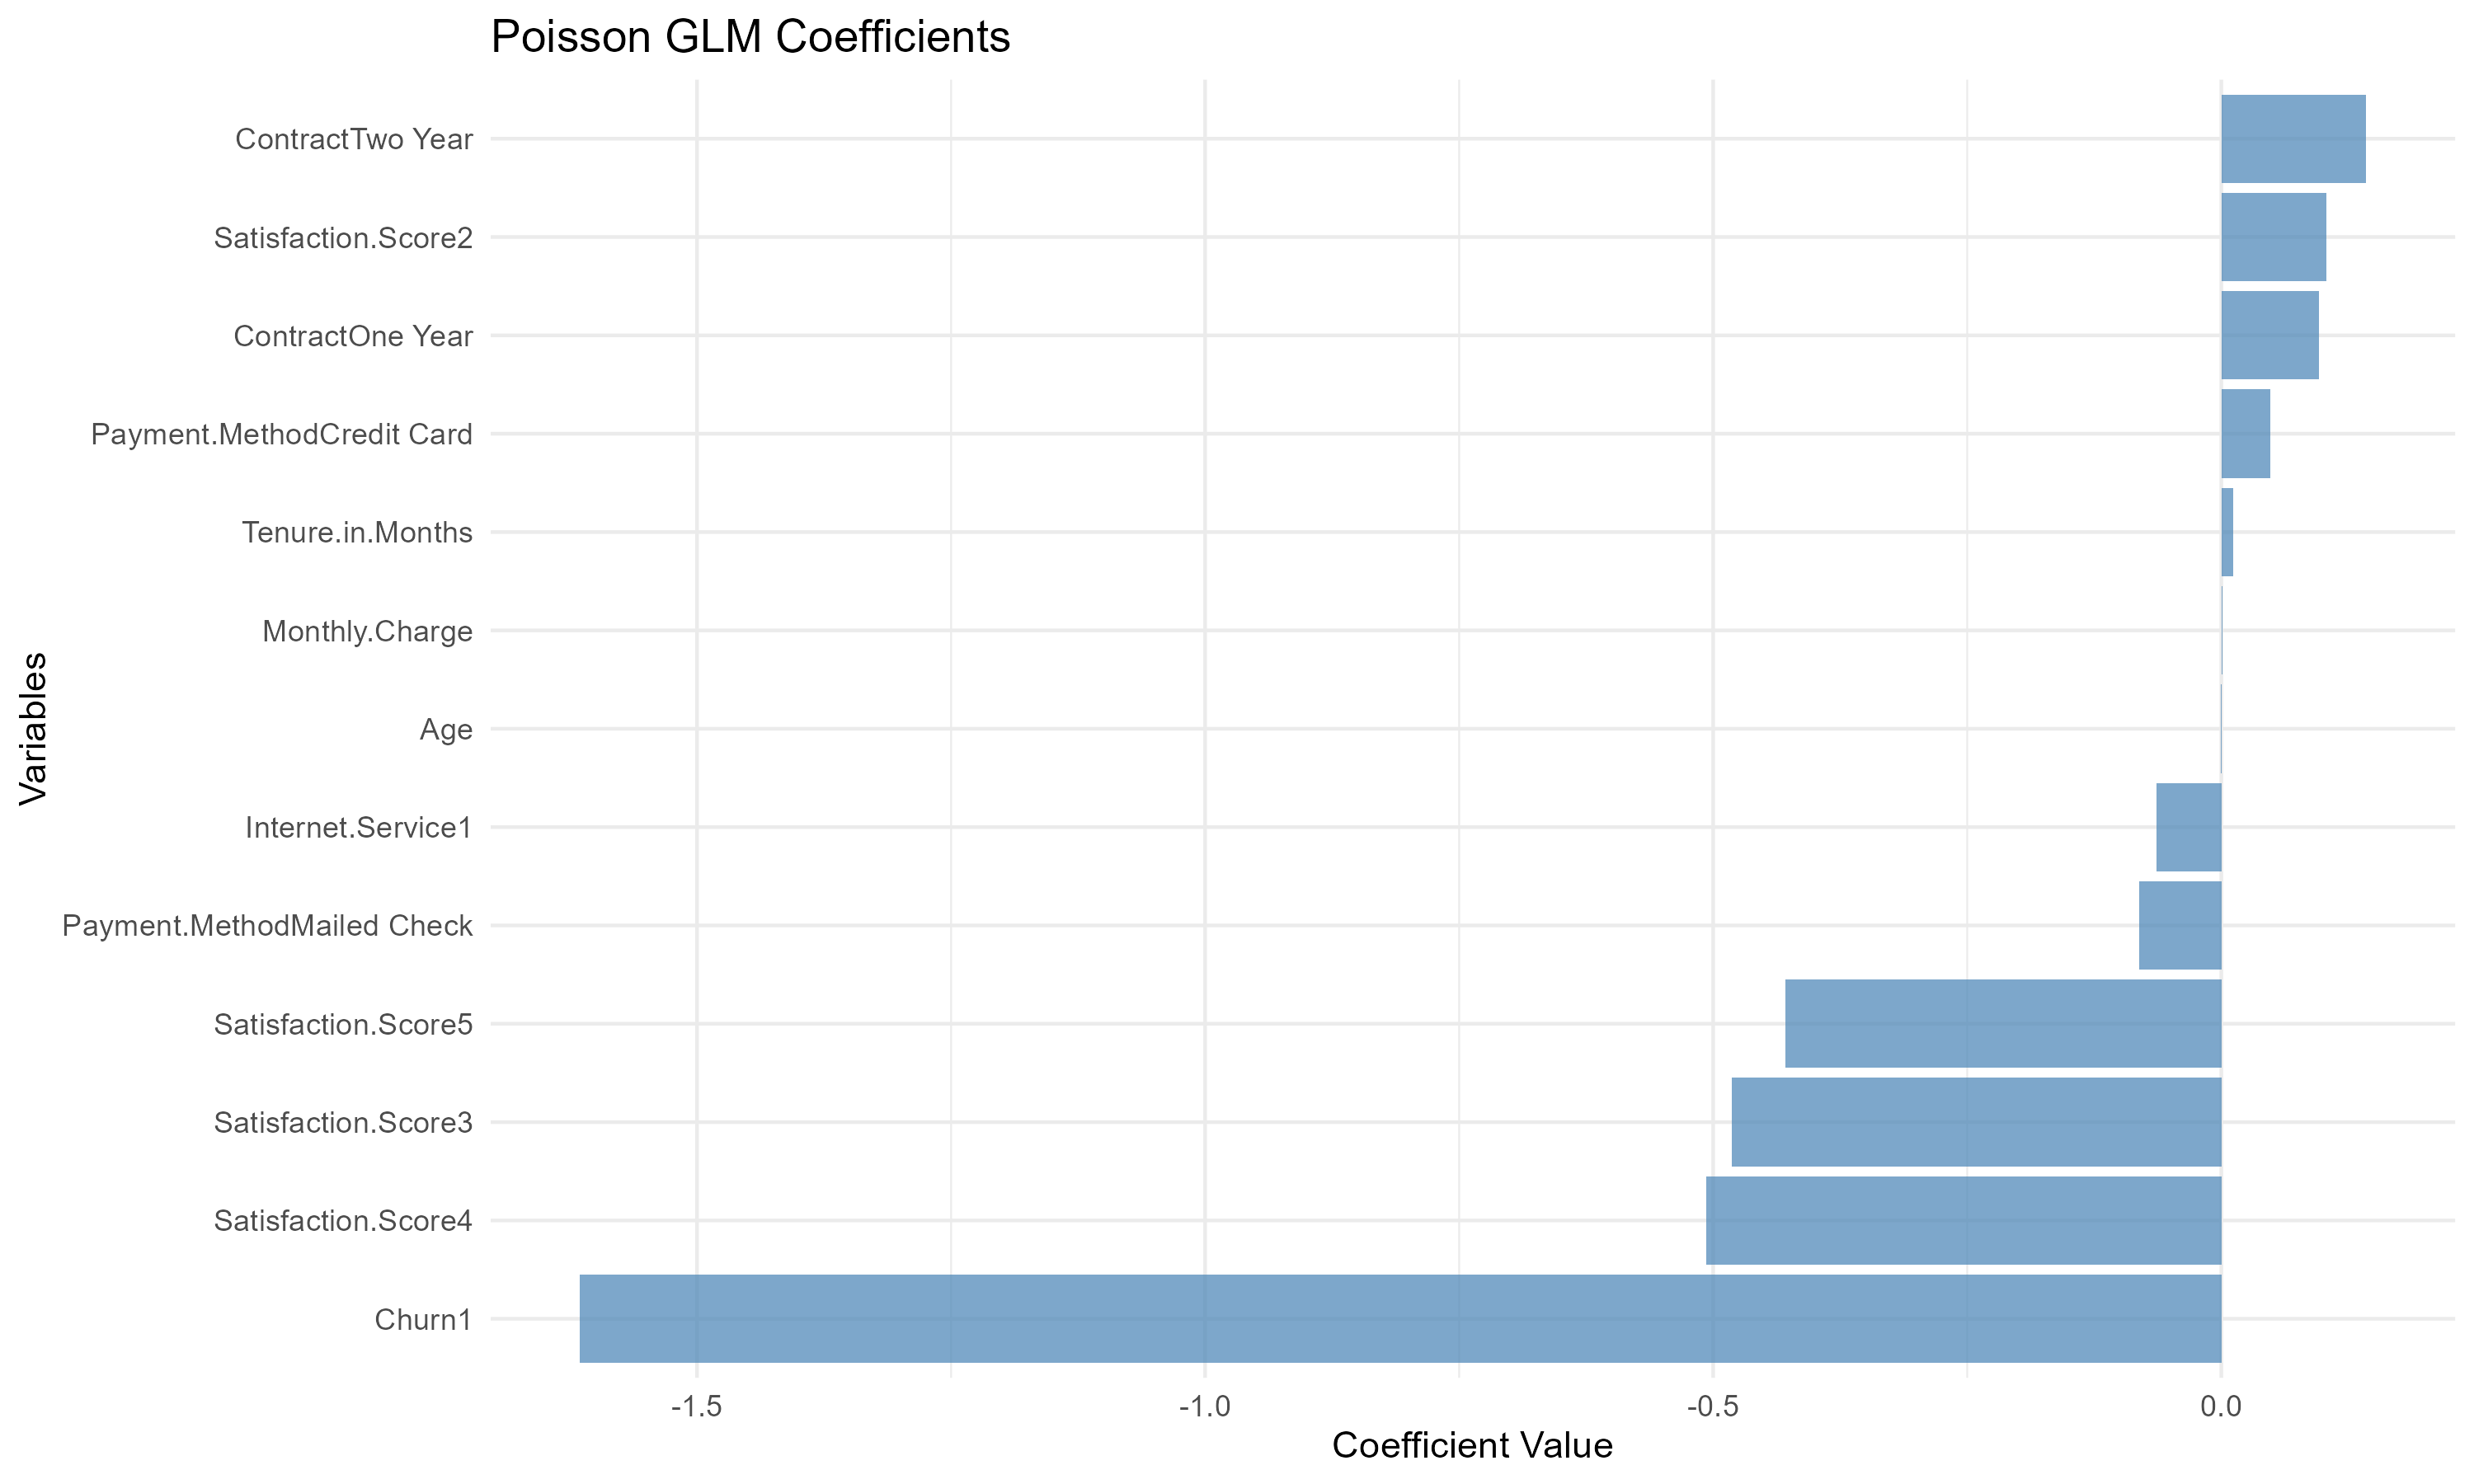
\includegraphics[width=0.8\linewidth]{Plots/poisson_coefficients} \end{center}

The coefficient plot reveals the substantial negative impact of customer
churn on referral behavior, with churned customers showing the largest
negative coefficient in the model. This finding reinforces the critical
business importance of retention strategies, as losing customers not
only eliminates direct revenue but also significantly reduces organic
customer acquisition through referrals. The magnitude of this effect
dwarfs other predictors, highlighting churn prevention as a dual-purpose
strategy for both revenue protection and marketing effectiveness.

\begin{center}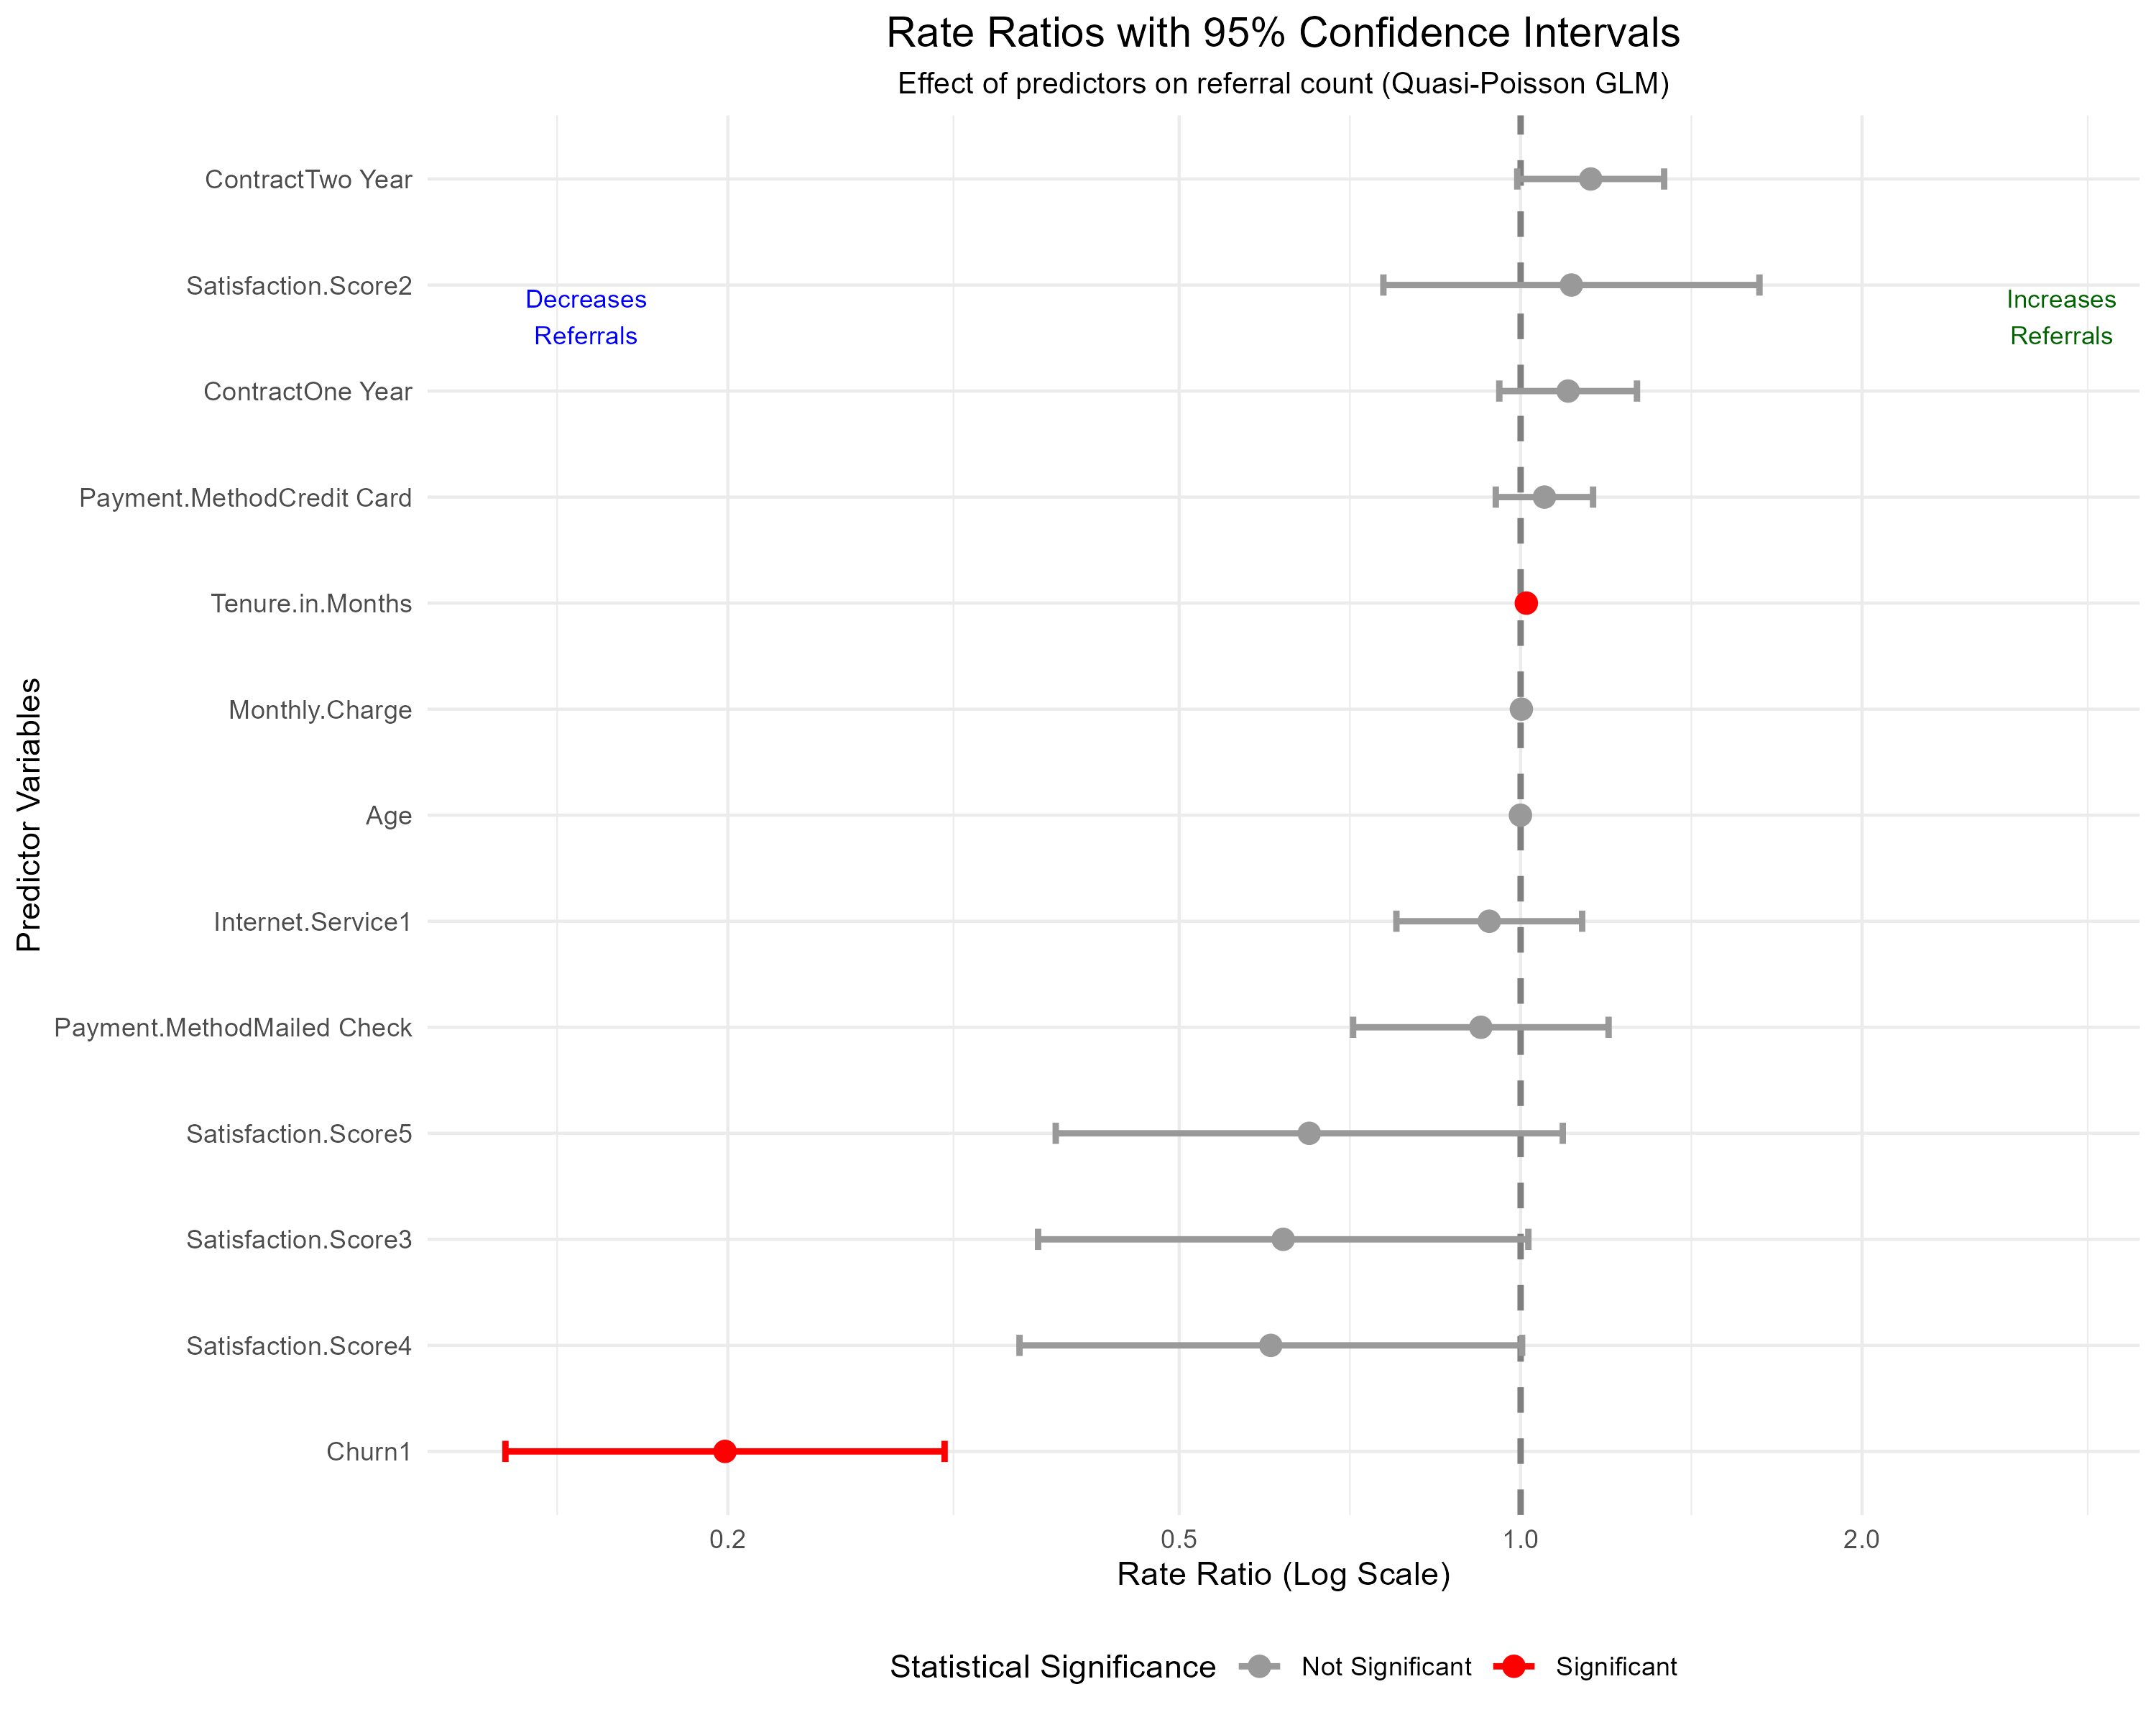
\includegraphics[width=0.8\linewidth]{Plots/poisson_forest_plot} \end{center}

The forest plot provides a comprehensive view of effect magnitudes with
their associated statistical uncertainty, enabling more nuanced
interpretation of predictor importance. The visualization clearly
demonstrates that tenure and churn status represent the most
statistically reliable predictors, with confidence intervals that do not
cross the null effect line at 1.0. Contract commitment effects show
meaningful positive associations with referral behavior, though with
wider confidence intervals reflecting greater uncertainty in these
estimates.

Satisfaction scores demonstrate interesting patterns, with scores 3, 4,
and 5 all showing negative coefficients of substantial magnitude. This
counterintuitive finding suggests that the relationship between
satisfaction and referral behavior may be more complex than initially
anticipated, potentially indicating that customers with moderate
satisfaction levels are more motivated to actively engage in referral
activities than those reporting the highest satisfaction scores.

Contract commitment variables show positive coefficients, with two-year
contracts demonstrating the strongest positive effect on referral
behavior. This pattern supports the business case for promoting
longer-term commitments, as these customers not only provide revenue
stability but also contribute more actively to customer acquisition
efforts. The tenure variable, while positive, shows a relatively modest
coefficient, indicating that while relationship length matters for
referrals, the effect accumulates gradually over time rather than
creating dramatic shifts in advocacy behavior.

\begin{longtable}[]{@{}lc@{}}
\caption{Cross-Validation Performance Summary}\tabularnewline
\toprule\noalign{}
Performance Metric & Result \\
\midrule\noalign{}
\endfirsthead
\toprule\noalign{}
Performance Metric & Result \\
\midrule\noalign{}
\endhead
\bottomrule\noalign{}
\endlastfoot
Mean RMSE across 5 folds & 2.8355 \\
Standard deviation & ±0.0582 \\
Performance consistency & High \\
Generalization capability & Good \\
\end{longtable}

Cross-validation analysis confirmed the model's stability and
generalization capability, with a mean RMSE of 2.8355 across five folds
and a standard deviation of 0.0582. This low variability in performance
across different data samples indicates that the model relationships are
robust and likely to maintain predictive accuracy when applied to new
customer populations.

The confusion matrix analysis for count predictions revealed the model's
ability to distinguish between different levels of referral activity.
While perfect prediction of exact referral counts remains challenging
due to the inherent variability in human behavior, the model
successfully identifies general referral propensity patterns that
support strategic decision-making for referral program design and
customer segmentation initiatives.

\hypertarget{business-applications-and-strategic-value}{%
\subsubsection{Business Applications and Strategic
Value}\label{business-applications-and-strategic-value}}

The Poisson GLM results enable several high-value business applications
that can directly impact customer acquisition costs and referral program
effectiveness. The model's identification of tenure as the strongest
predictor of referral behavior supports investment in retention
strategies as a dual-purpose initiative that both preserves existing
revenue and enhances organic customer acquisition through increased
referral activity.

Contract commitment insights provide clear guidance for product design
and customer engagement strategies. The positive relationship between
contract length and referral rates suggests that incentivizing
longer-term commitments not only improves revenue predictability but
also creates a more engaged customer base that actively promotes our
services. This finding supports the development of attractive long-term
contract offerings and retention incentives that encourage customers to
extend their commitment periods.

The satisfaction score patterns, while requiring further investigation,
highlight the importance of understanding customer sentiment dynamics
and their relationship to advocacy behavior. The results suggest that
referral program design should consider customer satisfaction levels
when targeting potential advocates, potentially focusing efforts on
customers with moderate satisfaction levels who may be most responsive
to referral incentives.

Payment method preferences also provide actionable insights, with credit
card users showing a 5.0\% increase in referral rates compared to other
payment methods. This finding suggests that customers who choose more
convenient payment options may also be more likely to engage in positive
word-of-mouth activities, supporting initiatives that encourage
electronic payment adoption.

\hypertarget{model-limitations-and-implementation-considerations}{%
\subsubsection{Model Limitations and Implementation
Considerations}\label{model-limitations-and-implementation-considerations}}

While the Poisson GLM provides valuable insights into referral behavior
patterns, successful implementation requires careful attention to
several important considerations. The substantial overdispersion
observed in the data indicates that referral behavior involves complex
factors beyond those captured in our current model. Future model
enhancements might consider additional variables such as social network
characteristics, geographic factors, or detailed service usage patterns
that could explain additional variance in referral behavior.

The model's temporal stability should be monitored regularly, as
customer behavior patterns and market conditions evolve continuously.
Quarterly model validation and annual recalibration procedures will help
ensure that coefficient estimates remain accurate and relevant for
strategic decision-making. Additionally, the satisfaction score
relationships warrant deeper investigation to understand the underlying
mechanisms driving the observed patterns.

The organization should also consider establishing clear protocols for
translating model insights into operational referral program decisions.
This includes developing guidelines for customer targeting based on
model predictions, setting appropriate incentive levels for different
customer segments, and measuring the business impact of model-driven
initiatives to validate the approach's effectiveness.

\hypertarget{conclusion}{%
\section{Conclusion}\label{conclusion}}

This study addressed Alphawave Telecom's critical challenge of reducing
their 24\% customer churn rate by investigating two key questions: which
factors drive customer churn most significantly, and which predictive
models deliver the highest accuracy for retention strategies. We
employed five distinct modeling approaches---Linear Models for CLTV
prediction, Support Vector Machines, Neural Networks, Poisson GLM for
referral behavior, and Generalized Additive Models---to provide both
interpretable insights and robust predictive capabilities.

Our analysis consistently identified satisfaction scores as the dominant
churn predictor across all modeling approaches, with correlation
coefficients exceeding 0.86 and demonstrating 94-97\% reduction in churn
likelihood for highly satisfied customers. Tenure in months emerged as
the second most critical factor, with polynomial analysis revealing a
vulnerable plateau phase between 10-30 months where proactive
intervention could prevent customer defection.

Predictive modeling revealed remarkably consistent performance across
methodologies. The optimized SVM classifier and neural network
architecture achieved approximately 98.6\% accuracy, while the logistic
GLM and GAM models demonstrated 95.4\% accuracy with superior
interpretability. Premium services (Online Security, Premium Tech
Support) showed 67-94\% lower churn odds, indicating these add-ons serve
as effective retention tools, while paperless billing customers
exhibited 85\% higher churn risk.

The logistic GLM emerged as the optimal operational model, balancing
accuracy (95.4\%), interpretability, and computational efficiency. The
two-layer neural network (6,4 neurons) provided complementary value for
complex pattern recognition, while the Poisson GLM offered actionable
insights for referral program optimization.

Several areas warrant further investigation to enhance the analytical
framework. The influential outliers identified through Cook's distance
analysis suggest potential customer microsegments that could benefit
from specialized modeling approaches. Integration of temporal dynamics
through survival analysis or time-series modeling could improve
understanding of churn timing and enable more precise intervention
scheduling.

Experimental validation of model recommendations through controlled
retention campaigns would provide valuable feedback for model
refinement. Additionally, deeper exploration of payment method
relationships with churn patterns, particularly under GDPR constraints,
could reveal additional retention opportunities. Finally, incorporating
real-time behavioral data streams could enhance model responsiveness and
prediction accuracy for dynamic customer intervention strategies.

\end{document}
